\documentclass[10pt,usenames,dvipsnames]{beamer}
\mode<presentation>
{
\usetheme{CambridgeUS}
\usecolortheme{dolphin}
}

\setbeamertemplate{footline}[frame number]
\definecolor{purple}{RGB}{255,0,204}

\usecolortheme[RGB={0,100,0}]{structure}

\AtBeginSection[]
{
  \begin{frame}<beamer>{Outline}
    \tableofcontents[currentsection,currentsubsection]
  \end{frame}
}

\usepackage{amsmath,amssymb,amsthm}
\usepackage{enumerate}
\usepackage{stfloats}
\usepackage{comment}

\usepackage{graphics} % for pdf, bitmapped graphics files
\usepackage{epsfig} % for postscript graphics files
\usepackage{mathptmx} % assumes new font selection scheme installed
\usepackage[mathscr]{euscript}
\usepackage{algorithm}
\usepackage[noend]{algpseudocode}

\makeatletter
\def\BState{\State\hskip-\ALG@thistlm}
\makeatother

\usepackage{tikz}
\usetikzlibrary{arrows,shapes,chains,matrix,positioning,scopes,patterns,calc}
\usepackage{pgfplots}
\usepgflibrary{shapes}

\newtheorem{remark}[theorem]{Remark}
\renewcommand{\epsilon}{\varepsilon}

\newcommand{\h}{\texttt{h}}
\newcommand{\hbp}{\h^{\mathrm{BP}}}
\newcommand{\hmap}{\h^{\mathrm{MAP}}}
\newcommand{\hstab}{\h^{\mathrm{stab}}}
\newcommand{\harea}{\h^{A}}
\newcommand\indep{\protect\mathpalette{\protect\independenT}{\perp}}
\def\independenT#1#2{\mathrel{\rlap{$#1#2$}\mkern2mu{#1#2}}}

\newcommand{\expt}{\mathbb{E}}
\newcommand{\indicator}[1]{\mathbbm{1}_{\left\{ {#1} \right\} }}
\newcommand{\abs}[1]{\left\lvert#1\right\rvert}

\newcommand{\mb}[1]{\mathbf{#1}}
\newcommand{\mbb}[1]{\mathbb{#1}}
\newcommand{\mr}[1]{\mathrm{#1}}
\newcommand{\mc}[1]{\mathcal{#1}}
\newcommand{\ms}[1]{\mathsf{#1}}
\newcommand{\msc}[1]{\mathscr{#1}}
\newcommand{\mf}[1]{\mathfrak{#1}}

\newcommand{\RNum}[1]{\uppercase\expandafter{\romannumeral #1\relax}}

\newcommand{\mse}{\mathsf{e}}
\newcommand{\msx}{\mathsf{x}}
\newcommand{\msxvn}{\tilde{\mathsf{x}}}
\newcommand{\msy}{\mathsf{y}}
\newcommand{\msz}{\mathsf{z}}
\newcommand{\msa}{\mathsf{a}}
\newcommand{\msb}{\mathsf{b}}
\newcommand{\msbx}{\underline{\mathsf{x}}}
\newcommand{\msby}{\underline{\mathsf{y}}}
\newcommand{\msbxvn}{\tilde{\underline{\mathsf{x}}}}
\newcommand{\msbz}{\underline{\mathsf{z}}}
\newcommand{\msba}{\underline{\mathsf{a}}}
\newcommand{\msbb}{\underline{\mathsf{b}}}
\newcommand{\msbc}{\underline{\mathsf{c}}}

%\newcommand{\bv}{\underline{\mathrm{b}}}
%\newcommand{\xv}{\underline{\mathrm{x}}}
%\newcommand{\yv}{\underline{\mathrm{y}}}
%\newcommand{\zv}{\underline{\mathrm{z}}}
%\newcommand{\rv}{\underline{\mathrm{r}}}
%\newcommand{\wv}{\underline{\mathrm{w}}}

%\newcommand{\Xv}{\underline{\mathrm{X}}}
%\newcommand{\Yv}{\underline{\mathrm{Y}}}
%\newcommand{\Zv}{\underline{\mathrm{Z}}}
%\newcommand{\Rv}{\underline{\mathrm{R}}}
%\newcommand{\RXYv}{\underline{\mathrm{R}_{XY}}}

\newcommand{\bv}{\vec{\mathrm{b}}}
\newcommand{\xv}{\vec{\mathrm{x}}}
\newcommand{\yv}{\vec{\mathrm{y}}}
\newcommand{\zv}{\vec{\mathrm{z}}}
\newcommand{\rv}{\vec{\mathrm{r}}}
\newcommand{\wv}{\vec{\mathrm{w}}}


\newcommand{\Xv}{\vec{X}}
\newcommand{\Yv}{\vec{Y}}
\newcommand{\Zv}{\vec{Z}}
\newcommand{\Rv}{\vec{R}}
\newcommand{\RXYv}{\vec{R}_{XY}}

\DeclareMathAlphabet{\mcl}{OMS}{cmsy}{m}{n}

\newcommand{\wh}{\widehat}
\newcommand{\bop}{\ast}
\newcommand{\vnop}{\varoast}
\newcommand{\disth}{d_{\mathrm{H}}}
\newcommand{\cnop}{\boxast}
\newcommand{\diff}[1]{d#1}
\newcommand{\deri}[1]{\mathrm{d}_{ #1 }\hspace{0.05cm}}
\newcommand{\dderi}[1]{\mathrm{d}_{ #1 }^2\hspace{0.05cm}}
\newcommand{\bvert}[1]{\,\Big{\vert}_{ #1  }}
\newcommand{\degr}{\succ}
\newcommand{\degreq}{\succeq}
\newcommand{\upgr}{\prec}
\newcommand{\upgreq}{\preceq}
\newcommand{\extR}{\overline{\mathbb{R}}}

\newcommand{\des}{\mathsf{T}_\mathrm{s}}
\newcommand{\dec}{\mathsf{T}_\mathrm{c}}
\newcommand{\pots}{U_\mathrm{s}}
\newcommand{\potc}{U_\mathrm{c}}
\newcommand{\shft}{\mathsf{S}}

\newcommand{\vnunit}{\Delta_0}
\newcommand{\cnunit}{\Delta_\infty}

\newcommand{\ent}[1]{ \mathrm{H} \left( #1 \right) }

\newcommand{\meass}{\mathcal{M}}
\newcommand{\probs}{\mathcal{X}}
\newcommand{\dpros}{\mathcal{X}_{\mathrm{d}}}
\newcommand{\chend}{N_{w}}

\newcommand{\minf}{\mathsf{a}_{0}}
\newcommand{\minfb}{\underline{\minf}}

\DeclareMathOperator*{\argmin}{\,arg\ min}
\DeclareMathOperator*{\argmax}{\,arg\ max}

\newlength\tikzwidth
\newlength\tikzheight

\textfloatsep=0.05in

\newcommand{\coleq}{\mathrel{\mathop:}=}
\newcommand{\defeq}{\triangleq}
\input{../../bib/avinash_beamer.def}

\def\figpath{../Figures}
\def\peeling_figpath{../Figures/peeling}
\def\mac_figpath{../Figures/MAC}
\def\cs_figpath{../Figures/CS}
\def\gt_figpath{../Figures/GT}

\begin{document}
\title{\bf Applications of coding theory to massive multiple access and big data problems}
\author{\textbf{Avinash Vem}\\ \vspace{3pt} \small Advisor: Dr.Krishna Narayanan} 
%\author{\textbf{Avinash Vem}\\ \vspace{3pt} \small Collaborators: Nagaraj Janakiraman, Dr. Krishna Narayanan\\\small Dr. J.-F. Chamberland, Dr. J. Cheng, Dr. Yu-Chih Huang} 
\vspace{5ex}
%\institute{Department of Electrical and Computer Engineering \\ Texas A\&M University}
\institute{Doctoral Degree Final Examination\\ Department of Electrical and Computer Engineering \\ Texas A\&M University}
\date{} % if no date wanted, keep it blank

%\titlegraphic{
%\includegraphics[width=0.5in]{\figpath/TAMULogoBox.pdf}
%}	

\frame{\titlepage}

%%%%%%%%%%%%----------------------------------------------------------------------------------%%%%%%%%%%%%%%%
\begin{frame}
\frametitle{Why massive multiple access?}

\begin{itemize}
\item 5G -- not just ``4G but faster'' but includes M2M transmissions, IoT
\item Current wireless -- a few devices with sustained data rate requirements
\item Future wireless -- {\color{blue}many uncoordinated} devices requiring {\color{blue}sporadic connectivity}
\item<2> Recent draft of IMT2020 - 1M devices per sq. km
\end{itemize}
\only<1>{
\centering
\includegraphics[width=0.9\textwidth]{\mac_figpath/5Gchanginglandscape.pdf}
}

\only<2>{
\centering
\includegraphics[width=0.7\textwidth]{\mac_figpath/IoT-application-ranking.png}
}
\end{frame}

%%%%%%%%%%%%----------------------------------------------------------------------------------%%%%%%%%%%%%%%%
\begin{frame}
\frametitle{Why compressed sensing and group testing}
\begin{itemize}
\setlength\itemsep{6pt}

	\item Generality of compressed sensing found use in wide variety of areas
	\begin{itemize}
	\setlength\itemsep{3pt}
 		\item measurements are costly e.g., MRI
		\item storage is expensive e.g., mobile phone camera sensor
		\item A/D converters, millimeter-wave holography etc.,
	\end{itemize}
	\item Applications of group testing include diverse fields like clone screening, human genome project, data forensics, finding shorts in circuits etc..,
\end{itemize}
\end{frame}

%%%%%%%%%%%%----------------------------------------------------------------------------------%%%%%%%%%%%%%%%
\begin{frame}\frametitle{Algorithmic complexity}
\centering
\resizebox{0.6\textwidth}{!}{\begin{tikzpicture}
\pgfkeys{/pgf/number format/set thousands separator = {}}
\begin{semilogyaxis}[%
font=\footnotesize,
width=3.5in,
height=2.9in,
xmajorgrids,
ymajorgrids,
title={Moore's Law versus Data Growth},
xlabel={Year},
legend entries={CPU Clock Frequency (MHz), Number of Cores, Number of Transistors (thousands), Mobile Data (GB/month), Computational Power, Data Growth},
legend style={fill=none},
legend style={draw=none},
legend cell align=left,
legend pos=north west
]

%Time, Frequency
\addplot [color=red, mark=*, only marks]
coordinates {
(1971.875,0.704135515) (1972.259615,0.509367522) (1974.326923,2.016914555) (1979.567308,5.048065717) (1982.307692,6.097562352) (1985.913462,16.10761535) (1986.25,16.10761535) (1988.653846,40.31519363) (1989.471154,24.80454414) (1990.576923,33.37624694) (1992.403846,65.52488237) (1992.692308,60.42963902) (1992.692308,100.9035045) (1993.028846,198.0956779) (1993.413462,67.31703824) (1993.413462,40.31519363) (1994.711538,151.2472545) (1994.711538,296.9314848) (1995.432692,296.9314848) (1995.721154,90.57977759) (1996.105769,198.0956779) (1996.346154,198.0956779) (1996.442308,90.57977759) (1996.826923,509.3675217) (1997.355769,252.5478933) (1997.451923,537.6117475) (1997.548077,232.9096592) (1997.644231,296.9314848) (1998.846154,495.8068242) (1999.134615,296.9314848) (1999.182692,399.5420559) (1999.471154,457.2526699) (1999.471154,509.3675217) (2000.192308,743.1795488) (2000.673077,1000) (2001.105769,897.6871324) (2001.201923,2016.914555) (2001.682692,805.8421878) (2001.778846,1420.18117) (2002.403846,2246.790092) (2002.788462,1810.558243) (2002.884615,1000) (2003.413462,1175.743266) (2003.509615,2186.974655) (2003.605769,1810.558243) (2004.807692,2641.64832) (2004.807692,1910.952975) (2004.855769,3651.741273) (2005.721154,3190.848981) (2005.865385,2788.126665) (2005.961538,1207.900747) (2006.009615,2246.790092) (2006.875,3651.741273) (2006.875,2641.64832) (2007.019231,2713.899431) (2007.067308,2308.241527) (2007.644231,2942.727176) (2007.740385,4655.525931) (2007.740385,4067.944321) (2007.836538,2016.914555) (2007.980769,1420.18117) (2008.173077,2016.914555) (2008.173077,2308.241527) (2008.461538,3023.213025) (2009.182692,2502.865431) (2009.278846,3278.121151) (2009.423077,2641.64832) (2009.663462,2641.64832) (2009.711538,3278.121151) (2010.192308,2308.241527) (2011.16,3470) (2011.32,2400) (2011.9,3000) (2012.4,3100) (2012.41,2900) (2012.7,3700) (2012.9,2500) (2013.4,1200) (2013.8,2700) (2014.16,2800) (2014.5,3700) (2014.8,3200) (2014.81,2600) (2014.82,2300) };

%Time, Cores
\addplot [color=cyan, mark=*, only marks]
coordinates {
(1971.875,1) (1972.259615,1) (1974.278846,1) (1979.615385,1) (1982.307692,1) (1985.913462,1) (1986.25,1) (1988.653846,1) (1989.471154,1) (1990.576923,1) (1992.355769,1) (1992.692308,1) (1992.980769,1) (1993.413462,1) (1994.711538,1) (1995.432692,1) (1995.769231,1) (1996.105769,1) (1996.490385,1) (1996.875,1) (1997.259615,1) (1997.451923,1) (1997.692308,1) (1998.846154,1) (1999.182692,1) (1999.519231,1) (2000.192308,1) (2000.673077,1) (2001.105769,1) (2001.634615,1) (2001.778846,1) (2002.355769,1) (2002.740385,1) (2002.932692,1) (2003.317308,1) (2003.509615,1) (2003.701923,1) (2004.807692,2) (2004.855769,1) (2005.721154,2) (2005.817308,1) (2005.961538,8) (2006.057692,2) (2006.826923,2) (2007.067308,2) (2007.644231,4) (2007.740385,9) (2007.740385,2) (2007.884615,2) (2007.980769,8) (2008.173077,4) (2008.461538,2) (2009.182692,3) (2009.230769,4) (2009.471154,4) (2009.615385,3) (2009.711538,8) (2009.711538,6) (2010.192308,16) (2011.16,12) (2011.32,20) (2011.9,8) (2012.4,16) (2012.41,16) (2012.7,32) (2012.9,16) (2013.4,240) (2013.8,24) (2014.16,30) (2014.5,64) (2014.8,16) (2014.81,24) (2014.82,36) };


%Time, Transistors
\addplot [color=blue, mark=*, only marks]
coordinates {
(1971.875,2.308241527) (1972.307692,3.554522356) (1974.326923,6.097562352) (1979.567308,29.16377574) (1982.307692,135.7727142) (1985.913462,273.8419634) (1986.25,109.4113811) (1988.653846,121.8814185) (1989.471154,1207.900747) (1990.576923,1207.900747) (1992.403846,1207.900747) (1992.692308,3105.900224) (1992.692308,1113.97386) (1993.028846,1715.437896) (1993.413462,3105.900224) (1993.413462,922.2395651) (1994.711538,1910.952975) (1994.711538,2788.126665) (1995.432692,9646.616199) (1995.721154,3105.900224) (1996.153846,5473.703263) (1996.346154,6792.52507) (1996.346154,3651.741273) (1996.442308,4293.51021) (1996.826923,9646.616199) (1997.355769,5473.703263) (1997.451923,3554.522356) (1997.548077,8896.491128) (1997.644231,7566.695371) (1998.894231,15261.37803) (1999.134615,9389.79801) (1999.182692,6978.305849) (1999.471154,9389.79801) (1999.471154,21673.9217) (2000.192308,22266.7201) (2000.673077,28387.35965) (2000.673077,37180.26664) (2001.105769,29163.77574) (2001.201923,42550.65502) (2001.682692,25482.96748) (2001.826923,37180.26664) (2002.403846,55730.60401) (2002.788462,38197.17549) (2002.884615,220673.4069) (2003.413462,151247.2545) (2003.509615,54246.90937) (2003.653846,106498.5635) (2004.807692,125214.9689) (2004.807692,106498.5635) (2004.807692,273841.9634) (2005.721154,232909.6592) (2005.817308,112403.8664) (2005.961538,305052.789) (2006.057692,115478.1985) (2006.875,378551.5249) (2006.875,155383.9831) (2006.923077,245824.4069) (2006.971154,296931.4848) (2006.971154,582941.5347) (2007.067308,151247.2545) (2007.644231,582941.5347) (2007.740385,232909.6592) (2007.788462,805842.1878) (2007.836538,115478.1985) (2007.980769,509367.5217) (2008.221154,445079.4062) (2008.461538,410469.838) (2009.182692,457252.6699) (2009.278846,784388.5581) (2009.663462,2308241.527) (2009.711538,1910952.975) (2010.192308,410469.838) (2010.384615,1309747.264) (2011.16,1170000) (2011.32,2600000) (2011.9,1200000) (2012.4,2400000) (2012.41,2300000) (2012.7,2100000) (2012.9,1200000) (2013.4,5000000) (2013.8,4300000) (2014.16,4300000) (2014.5,4200000) (2014.8,2600000) (2014.81,3800000) (2014.82,5700000) };

\addplot [color=black, mark=*, only marks]
coordinates {
(2009, 91000000) (2010, 220000000) (2011, 402000000) (2012, 884000000) (2013, 1480000000) (2014, 2514000000) (2015, 3685000000) (2016, 7241000000) (2017, 11266000000) (2018, 16792000000) (2019, 24452000000) (2020, 34588000000) };

\addplot [color=blue, densely dashed, line width=1.2pt]
coordinates {
(1972, 1.42192406e+00) (1973, 2.01272654e+00) (1974, 2.84900455e+00) (1975, 4.03275198e+00) (1976, 5.70834066e+00) (1977, 8.08012823e+00) (1978, 1.14373819e+01) (1979, 1.61895580e+01) (1980, 2.29162401e+01) (1981, 3.24378255e+01) (1982, 4.59155830e+01) (1983, 6.49932828e+01) (1984, 9.19976733e+01) (1985, 1.30222256e+02) (1986, 1.84328965e+02) (1987, 2.60916746e+02) (1988, 3.69326375e+02) (1989, 5.22779674e+02) (1990, 7.39992067e+02) (1991, 1.04745514e+03) (1992, 1.48266762e+03) (1993, 2.09870875e+03) (1994, 2.97071196e+03) (1995, 4.20502822e+03) (1996, 5.95219683e+03) (1997, 8.42530545e+03) (1998, 1.19259786e+04) (1999, 1.68811642e+04) (2000, 2.38952052e+04) (2001, 3.38235459e+04) (2002, 4.78770634e+04) (2003, 6.77697486e+04) (2004, 9.59277471e+04) (2005, 1.35785256e+05) (2006, 1.92203364e+05) (2007, 2.72062920e+05) (2008, 3.85103730e+05) (2009, 5.45112443e+05) (2010, 7.71603991e+05) (2011, 1.09220167e+06) (2012, 1.54600611e+06) (2013, 2.18836407e+06) (2014, 3.09761862e+06) (2015, 4.38466397e+06) (2016, 6.20647036e+06) (2017, 8.78522838e+06) (2018, 1.24354477e+07) (2019, 1.76023153e+07)};

\addplot [color=black, densely dashed, line width=1.2pt]
coordinates {
(1990, 5.96878326e+03) (1991, 1.01461770e+04) (1992, 1.72472182e+04) (1993, 2.93180907e+04) (1994, 4.98370478e+04) (1995, 8.47166811e+04) (1996, 1.44007648e+05) (1997, 2.44794797e+05) (1998, 4.16120209e+05) (1999, 7.07351751e+05) (2000, 1.20240856e+06) (2001, 2.04394254e+06) (2002, 3.47444393e+06) (2003, 5.90611546e+06) (2004, 1.00396496e+07) (2005, 1.70661352e+07) (2006, 2.90102724e+07) (2007, 4.93137958e+07) (2008, 8.38272187e+07) (2009, 1.42495675e+08) (2010, 2.42224633e+08) (2011, 4.11751255e+08) (2012, 6.99925082e+08) (2013, 1.18978416e+09) (2014, 2.02248266e+09) (2015, 3.43796485e+09) (2016, 5.84410562e+09) (2017, 9.93424077e+09) (2018, 1.68869535e+10) (2019, 2.87056861e+10) };

\end{semilogyaxis}
\end{tikzpicture}}

\begin{itemize}
\item<2> Linear complexity is too expensive, sub-linear complexity is required
\end{itemize}
\end{frame}


%%%%%%%%%%%%----------------------------------------------------------------------------------%%%%%%%%%%%%%%%
\begin{frame}
\frametitle{Outline}
\begin{itemize}
\setlength{\itemsep}{6pt}
\item \emph{Unsourced, uncoordinated} massive multiple access
%\begin{itemize}
%\item interested only in \emph{what} is transmitted, not \emph{who}
%\end{itemize}
\item Compressed sensing: support recovery
\item Non-adaptive group testing: \emph{approximate} and \emph{probabilistic}
\end{itemize}
\centering
\resizebox{0.5\textwidth}{!}{\input{\figpath/venn_theme.tex}}
\end{frame}

%%%%%%%%%%%%----------------------------------------------------------------------------------%%%%%%%%%%%%%%%
\begin{frame} 
\frametitle{Common theme}
\begin{itemize}
	\setlength{\itemsep}{4pt}
%	\item {\color{blue}Sparsity}
%	\begin{itemize}
%	\setlength{\itemsep}{3pt}
%		\item Number of users active $\ll$ total number of users in the system
%		\item Sensing signal is sparse in some domain
%		\item Defective items to be identified $\ll$ number of items
%	\end{itemize}
%	\pause
	\item Coding schemes based on {\color{blue}bipartite Tanner graphs} leveraging the inherent sparsity
	\item<2-> {\color{blue} Iterative peeling}-like algorithms used for decoding/recovery 
	\item<2-> Importantly the {\color{blue} computational complexity scales with sparsity} of the problem
\end{itemize}
\centering
\resizebox{0.5\textwidth}{!}{\begin{tikzpicture}
\def\fsize{\footnotesize}

	\def \r{2.5cm}
	\def\firstcircle{(90:1.65cm) circle (\r)}
  	\def\secondcircle{(210:1.65cm) circle (\r)}
	 \def\thirdcircle{(330:1.65cm) circle (\r)}
  
     \draw \firstcircle node[text=black,anchor=south] {
         \fsize{\begin{tabular}{c}
	 Unsourced MAC\\
	no. active users $\ll$ no. users\\
    \end{tabular}}
     };
     
    \draw \secondcircle node[text=black,anchor=north east] { %\fsize{Compressed sesning}};
    \fsize{\begin{tabular}{c}
    Compressed \\
    sensing\\
    \end{tabular}}
    };
    \draw \thirdcircle node[text=black,anchor=north west] {
        \fsize{\begin{tabular}{c}
	Group\\ testing\\ 
  \end{tabular}}
};
  
   \begin{scope}
    \clip \firstcircle;
    \clip \secondcircle;
    \fill[gray] \thirdcircle;
      \end{scope}

  \end{tikzpicture}}
\end{frame}

%%%%%%%%%%%%----------------------------------------------------------------------------------%%%%%%%%%%%%%%%
\begin{frame}
	\frametitle{Outline}
	\tableofcontents
\end{frame}


\section{Peeling decoder}
\subsection{LDPC Code}

\begin{frame}\frametitle{Tanner Graph - LDPC Code}
\begin{columns}

\column{0.45\textwidth}
\begin{defn}{Parity-Check Matrix}
\centering
\begin{align*}
H=
\begin{pmatrix}
1 & 0 & 1 & 1 & 0 & 0\\
1 & 1 & 0 & 0 & 1 & 0\\
0 & 1 & 1 & 0 & 0 & 1
\end{pmatrix}
\end{align*}
\vspace{6ex}
\begin{align*}
\text{LDPC Code } \mc{C}=\{x: H\odot x=0 \}
\end{align*}
\end{defn}

\pause

\column{0.45\textwidth}
\begin{defn}{Tanner Graph}
\centering
\vspace{0.6cm}
\resizebox{\textwidth}{!}{\begin{tikzpicture}
\def\horzgap{7ex}; %Horizontal gap between nodes/levels
\def \gapVN{4ex}; %vertical gap between variable nodes
\def \gapCN{6ex}; %Horizontal gap between check nodes
\def\nodewidth{1.5ex};

\def \textoffs{1ex}; %Offset for writing text east of a node
%\def\nodewidthA{0.05in};
%\def \edgewidth{0.02in};
%\def\ext{0.2in};
`
\def \n{8};
\def\ldeg{2};
\def \m {4};
\def\rdeg{3};

\def\langle{40};%120 degrees/3
\def\langle{20};%120 degrees/6

\tikzstyle{check} = [rectangle, draw, line width=0.75pt, inner sep=0mm, minimum height=\nodewidth, minimum width=\nodewidth]
\tikzstyle{bit} = [circle, draw,line width=0.75pt, inner sep=0mm, minimum size=\nodewidth]

                          
\foreach \vn in {1,...,6}{
 \node[bit] (vn\vn) at (0,-\vn*\gapVN) {\footnotesize $x_{\vn}$};
}


\foreach \cn in {1,...,3}{
\node[check] (cn\cn) at (\horzgap,-0.2*\gapCN-\cn*\gapCN) {};
}

\path (cn1.east)++(\textoffs,0) node ()[anchor=west] {\tiny{$x_1\oplus x_3\oplus x_4=0$}};

%\draw (vn6.east)--(cn4.west);
%\draw (vn3.east)--(cn4.west);
%\draw (vn1.east)--(cn4.west);

%\draw(vn2.east)--(cn3.west);
%\draw (vn4.east)--(cn3.west);
%\draw(vn5.east)--(cn3.west);

\draw (vn2.east)--(cn3.west);
\draw (vn3.east)--(cn3.west);
\draw  (vn6.east)--(cn3.west);

\draw (vn1.east)--(cn2.west);
\draw (vn2.east)--(cn2.west);
\draw (vn5.east)--(cn2.west);

\draw (vn1.east)--(cn1.west);
\draw (vn3.east)--(cn1.west);
\draw (vn4.east)--(cn1.west);

\node () at (0,-6.5*\gapVN){\tiny Variable Nodes};
\node () at (1.1*\horzgap,-3.5*\gapCN){\tiny Check Nodes};

\end{tikzpicture}}
\end{defn}

\end{columns}
\end{frame}

%--------------------------12314yoi34u9123092u308912------------------------------
\subsection{Decoder-BEC Channel}
\begin{frame}
\frametitle{Iterative peeling process}
\begin{columns}
\column{0.4\textwidth}
\begin{align*}
x_1\oplus x_3\oplus x_4&=0\\
x_1\oplus x_2\oplus x_5&=0\\
x_2\oplus x_3\oplus x_5&=0
\end{align*}

\vspace{0.2cm}
\centering
\only<2->{\includegraphics[scale=0.15,angle=270]{\figpath/BECchannelmodel.pdf}}

\column{0.6\textwidth}
\resizebox{0.9\textwidth}{!}{\pgfdeclarelayer{background}
\pgfdeclarelayer{foreground}
\pgfdeclarelayer{m-f}
\pgfdeclarelayer{main}

\pgfsetlayers{background,foreground}
\colorlet{LightBlue}{blue!10!white}
\colorlet{DarkBlue}{blue!80!white}

\begin{tikzpicture}[scale=1.0]
\clip (-0.15in,0.15in) rectangle (1.3in,-2.5in);

\def\n     {6}   % #-Variable nodes
\def\m     {3}  % #-Check nodes
\def\nodewidth{0.15in}
\def\nodegapVN{0.3in}
\def\nodegapCN{0.5in}

\tikzstyle{check} = [rectangle, draw, text centered, thick, fill=red,
                          minimum height=\nodewidth, minimum width=\nodewidth]
\tikzstyle{bit} = [circle, draw, text centered, thick, fill=LightBlue,
                          radius=0.5*\nodewidth]
\tikzstyle{bitpeeled} = [circle, draw, text centered, thick, fill=DarkBlue,
                          radius=0.5*\nodewidth]

\begin{pgfonlayer}{background}
%\draw[gray,step=0.5in] (-0.15in,0.15in) grid (1.5in,-2.5in);
\foreach \vn in {1,...,\n}{
  \node[bit] (vn\vn) at (0,-\vn*\nodegapVN) {};
 }

 \foreach \cn in {1,...,\m}{
  \node[check] (cn\cn) at (1in,-\cn*\nodegapCN) {};
 }
\end{pgfonlayer}



\begin{pgfonlayer}{foreground}

%Text to left of VN
\only<1>{
\foreach \vn in {1,...,\n}{
  \node[left] (nodetxt) at (vn\vn.west) {\normalsize{$x_\vn$}};
 	}  	
}

\only<2-8>{
\foreach \vn/\txt in {2/1,4/1,5/0}{
\node[left] (nodetxt) at (vn\vn.west) {\normalsize{\txt}};
 	}	
}

\only<2-3>\node[left] (nodetxt) at (vn1.west) {\normalsize{E}};
\only<2-5>\node[left] (nodetxt) at (vn3.west) {\normalsize{E}};
\only<2-7>\node[left] (nodetxt) at (vn6.west) {\normalsize{E}};


\only<4-8>\node[left] (nodetxt) at (vn1.west) {\normalsize{E=1}};
\only<6-8>\node[left] (nodetxt) at (vn3.west) {\normalsize{E=0}};
\only<8>\node[left] (nodetxt) at (vn6.west) {\normalsize{E=1}};

%Edges
\uncover<1-2>{
\foreach \vn/\cn in {2/2,2/3,4/1,5/2}{
 \draw[thick] (vn\vn.east)--(cn\cn.west);
  }
}

\only<1-3>\draw[thick] (vn1.east)--(cn2.west);
\only<1-4>\draw[thick] (vn1.east)--(cn1.west);

\only<1-5>\draw[thick] (vn3.east)--(cn1.west);
\only<1-6>\draw[thick] (vn3.east)--(cn3.west);

\only<1-5>\draw[thick] (vn3.east)--(cn1.west);
\only<1-6>\draw[thick] (vn3.east)--(cn3.west);

\only<1-7> \draw[thick] (vn6.east)--(cn3.west);

%% Peeled bits color
\uncover<3-8>{
  \foreach \vn in {2,4,5}{
    \node[bitpeeled] () at (vn\vn) {};
    }
  }
 \only<4-8>\node[bitpeeled] () at (vn1) {};
 \only<6-8>\node[bitpeeled] () at (vn3) {};
  \only<8>\node[bitpeeled] () at (vn6) {};

%Check node values
\only<2,5,6,7,8> \node[right] (nodetxt) at (cn1.east) {\normalsize{0}};
\only<3,4> \node[right] (nodetxt) at (cn1.east) {\normalsize{1}};

\only<2,4,5,6,7,8> \node[right] (nodetxt) at (cn2.east) {\normalsize{0}};
\only<3> \node[right] (nodetxt) at (cn2.east) {\normalsize{1}};

\only<2,6,7,8> \node[right] (nodetxt) at (cn3.east) {\normalsize{0}};
\only<3,4,5> \node[right] (nodetxt) at (cn3.east) {\normalsize{1}};



%% Text at the bottom
\only<1> \node[minimum width=10cm] (txt) at (0.5in,-7*\nodegapVN) {Tanner Graph};
\only<2> \node[minimum width=10cm] (txt) at (0.5in,-7*\nodegapVN) {Received block};
\only<3> \node[minimum width=10cm] (txt) at (0.5in,-7*\nodegapVN) {Peeling Step 1};
\only<4-5> \node[minimum width=10cm] (txt) at (0.5in,-7*\nodegapVN) {Peeling Step 2};
\only<6-7> \node[minimum width=10cm] (txt) at (0.5in,-7*\nodegapVN) {Peeling Step 3};
\only<8> \node[minimum width=10cm] (txt) at (0.5in,-7*\nodegapVN) {Peeling Step 4};

\end{pgfonlayer}
\end{tikzpicture} }
\end{columns}
\end{frame}

%--------------------------12314yoi34u9123092u308912------------------------------
\begin{frame}\frametitle{Threshold behavior}
\begin{columns}
\column{0.45\textwidth}
\begin{defn}{Threshold behavior}
\begin{itemize}
\item $N$-variable nodes, $m$-check nodes %$\epsilon$-erasure probability
\item If $m=\alpha N$ scales linearly, $\exists \alpha^{*}$
\begin{align*}
\lim_{N\rightarrow \infty}\Pr(\mc{E})=0 ~~ \text{ if }\alpha>\alpha^*
\end{align*}
\item $\Pr(\mc{E})>0$ if $\alpha<\alpha^*$
\end{itemize}
\end{defn}

\pause

\column{0.55\textwidth}
\includegraphics[width=\textwidth]{\figpath/BEC_MCT.png}
\begin{itemize}
\item $\Pr(\mc{E})$ for (3,6) d.d. for $N=2^i, i=6,\ldots,20$.  $m=N/2$
\end{itemize}

\end{columns}
\end{frame}

%--------------------------12314yoi34u9123092u308912------------------------------
\begin{frame}\frametitle{General framework}
\begin{columns}
\column{0.4\textwidth}
\resizebox{\textwidth}{!}{\begin{tikzpicture}
\def\horzgap{7ex}; %Horizontal gap between nodes/levels
\def \gapVN{4ex}; %vertical gap between variable nodes
\def \gapCN{5ex}; %Horizontal gap between check nodes
\def\nodewidth{1.5ex};

\def \textoffs{1ex}; %Offset for writing text east of a node
%\def\nodewidthA{0.05in};
%\def \edgewidth{0.02in};
%\def\ext{0.2in};
`
\def \n{8};
\def\ldeg{2};
\def \m {4};
\def\rdeg{3};

\def\langle{40};%120 degrees/3
\def\langle{20};%120 degrees/6

\tikzstyle{check} = [rectangle, draw, line width=0.75pt, inner sep=0mm, minimum height=\nodewidth, minimum width=\nodewidth]
\tikzstyle{bit} = [circle, draw,line width=0.75pt, inner sep=0mm, minimum size=\nodewidth]

                          
\foreach \vn in {1,...,6}{
 \node[bit] (vn\vn) at (0,-\vn*\gapVN) {};
}


\foreach \cn in {1,...,4}{
\node[check] (cn\cn) at (\horzgap,-0.1*\gapCN-\cn*\gapCN) {\tiny{$f()$}};
}

\path (cn2)++(0,-0.4*\gapCN) node () {\small{$\vdots$}};

\path (cn1.east) node[anchor=west] (ytexta) {\tiny{$y_1=f(\{x_i\})$}};
\path (ytexta) node[anchor=north] () {\tiny{$i\in\mc{N}_1$}};

%\path (cn4.east) node[anchor=west] () {\tiny{$y_m=f(\{x_i,i\in\mc{N}_m\})$}};

\path (cn4.east) node[anchor=west] (ytextb) {\tiny{$y_m=f(\{x_i\})$}};
\path (ytextb) node[anchor=north] () {\tiny{$i\in\mc{N}_m$}};


\draw (vn4.east)--(cn4.west);
\draw  (vn5.east)--(cn4.west);

\draw (vn2.east)--(cn3.west);
\draw (vn3.east)--(cn3.west);
\draw  (vn6.east)--(cn3.west);

\draw (vn1.east)--(cn2.west);
\draw (vn2.east)--(cn2.west);
\draw (vn5.east)--(cn2.west);

\draw (vn1.east)--(cn1.west);
\draw (vn3.east)--(cn1.west);
\draw (vn4.east)--(cn1.west);

%\node[text width=1.5cm] () at (0,-6.5*\gapVN){\tiny $N$ Variable Nodes $K$ unknown};
\node[align=left] () at (0,-6.5*\gapVN){\tiny $N$ Variable Nodes};
\node[align=left] () at (0,-6.8*\gapVN){\tiny $K$ unknown};
\node () at (1.2*\horzgap,-4.6*\gapCN){\tiny $m$ Function Nodes};

\end{tikzpicture}}

\column{0.6\textwidth}
\begin{itemize}
\item Need to recover $K$ unknowns$/N$ variables
\item We know values of $m$ functions $y_1,\ldots,y_m$
\item via peeling decoder, $m=cK$ sufficient {\tiny ($c>1$)}
\end{itemize}
\pause
\vspace{5ex}
\begin{itemize}
\item $c$ depends on the d.d of the graph, can be evaluated analytically via DE
\item $f$ amenable for peeling
\end{itemize}

\end{columns}
\end{frame}


\section{Unsourced multiple access}
\subsection{Problem statement}
%%%%%%%%%%%%----------------------------------------------------------------------------------%%%%%%%%%%%%%%%
\begin{frame} \frametitle{Multiple access - Over the years}

\begin{itemize}
\setlength{\itemsep}{3ex}
   \item Information-theoretic view (asymptotic in blocklength)
\begin{itemize}
\item  Liao-1972
\item {[Ahlswede-1973]} Capacity of 2 $\&$ 3-user MAC 
\end{itemize}

   \item Network-theoretic view (random access strategy)
	\begin{itemize}
		\item {[Abramson 1970]} ALOHA random access
		\item {[Cassini 2007]} Contention-resolution diversity slotted ALOHA
	\end{itemize}
	
	\item Coding-theoretic view (coordinated, small number of users)
		\begin{itemize}
		\item  CDMA, multi-user detection
		\item {[Chang,Weldon 1979; Wolf 1981]} $T$-user adder MAC 
	\end{itemize}
	\pause

	\item Unsourced uncoordinated MAC (Polyanskiy 2017)
		\begin{itemize}
			\item For the first time, considered the three point-of-views together: 
			\begin{itemize}
				\item small payload; \emph{finite block length, uncoordinated}
				\item a large number of users in the system \emph{unsourced, massive}
				\item power constraint 
				\item finite number of users active at a given time \emph{sporadic connectivity}
			\end{itemize}
	   \end{itemize}
\end{itemize}
\end{frame}

%%%%%%%%%%%%----------------------------------------------------------------------------------%%%%%%%%%%%%%%%
\begin{frame}
\frametitle{System Model}

\begin{itemize}
  \item $N$ \textbf{uncoordinated} users present in the system
  \item $K$ users \textbf{active} at any given time. Each user has 1 packet to transmit
  \item Time frame is \textbf{slotted}, transmissions occur in slots
   \begin{itemize}
	   \item In slot $j$, each user can choose to transmit or not
	\end{itemize}
   \item<2-> BS interested only in the \textbf{set} of packets, not the \textbf{source}
	\begin{itemize}
	   \item<2-> Due to small payload and a large number of users ($N\gg K$)
	 \end{itemize}
   
\end{itemize}

 \begin{center}
  \input{\mac_figpath/slots}
  \end{center}
\end{frame}

%%%%%%%%%%%%----------------------------------------------------------------------------------%%%%%%%%%%%%%%%
\begin{frame}\frametitle{Problem statement}
  \begin{itemize}
  \setlength{\itemsep}{3pt}
  \item $N$ users out of which $K$ active. $K\in[25:300]$
  \item Each user has a $B$-bit message. $B$ is small $\approx 100$
  \item $n=30,000$ channel uses available per round
  \item {\small regime of interest for LP-WANs such as LoRaWAN, Weightless}
\end{itemize}
  \pause
  \vspace{2ex}

  \begin{itemize}
  \item $\{w_1,w_2,\ldots,w_K\}$ - set of messages to be transmitted
  \item Power constraint -$~\frac{1}{n}\mathbb{E}_w[||\xv_w||^2]\leq P$
  \item Channel model $\yv=\sum_{j=1,\ldots,K}\xv_{w_j}+\zv$. $\vec{z}\sim\mc{N}(0,\mathbf{I}_n)$
  \item If $\mc{L}(\yv)=\{\hat{w}_1,\ldots,\hat{w}_K\}$ is the decoder output, $P_e=\frac{1}{K}\sum\limits_{i=1}^{K} \Pr\left( w_i \notin \mc{L}(\yv) \right) $
  \end{itemize}
      \pause
      \vspace{3ex}
  \begin{block}{Objective}
 Design a coding scheme minimizing the required SNR $P$ such that 
 \begin{itemize}
 \item the encoding and decoding complexities are polynomial in $K,n$ and $B$
 \item prob. of decoding error per user $P_e\leq \epsilon\in [0.05,0.1]$
\end{itemize} 
  \end{block}
 
\end{frame}

%%%%%%%%%%%%----------------------------------------------------------------------------------%%%%%%%%%%%%%%%
\begin{frame} \frametitle{Multiple access - Over the years}
	\begin{itemize} 
	\item {[Polyanskiy 2017]} Gaussian coding for unsourced MAC 
	\vspace{3pt}
	\begin{itemize}	\setlength{\itemsep}{4pt}
		\item Derived achievability limits via random Gaussian coding 
			\begin{itemize}
				\item MMSE decoder: {\color{red} exponential complexity} in $B,K$. $\mc{O}(n\cdot\binom{2^B}{K})\approx\mc{O}(n2^{BK})$
			\end{itemize}
			\item In comparison, ALOHA, TIN found to be very energy-inefficient for $K\gtrapprox100$
	\end{itemize}
	\pause 
	\vspace{4ex}
	\item {[OP-2017]} Low complexity coding scheme for unsourced MAC
	\begin{itemize}\setlength{\itemsep}{4pt}
		\item Concatenated code for $T$-GMAC: Integer forcing and mod-$2$ addition MAC 
		\item {\color{blue} polynomial} encoding and decoding complexity $\mc{O}\left(\max(n, KB^2)\right)$
		\item {\color{blue} outperforms} existing strategies, however {\color{red} $\approx 20dB$ away} from [YP17] ach. limit
		\pause
		\begin{itemize}	\setlength{\itemsep}{2pt}
		\item sub-optimal coding scheme for the $T$-user real adder GMAC
		\item ``capacity achieving low complexity \emph{same-codebook} schemes for the $T$-GMAC channel seems to be a challenging task"
		\item absence of iterative successive interference cancellation(SIC)
		\end{itemize}
	\end{itemize}
\end{itemize}
\end{frame}

%%%%%%%%%%%%----------------------------------------------------------------------------------%%%%%%%%%%%%%%%
\begin{frame}\frametitle{Main Result}
\only<1-2>{
Main features of the proposed scheme:
\begin{itemize}
\item Same codebook for all the users. Encoder solely depends on the message
\item Two stages of encoding:
	\begin{itemize}
	\setlength{\itemsep}{2pt}
	\item encoder within a slot: Code with close to optimal performance for $T$-GMAC
	\item encoder across slots: above codeword is repeated in multiple slots
    \item repetition pattern is dependent solely on the message
	\end{itemize}
\item Peeling based successive interference cancellation(SIC) decoding across slots
\end{itemize}
}
\only<3>{
\centering
\resizebox{0.55\textwidth}{!}{\input{\mac_figpath/sim_results_nomark}}
}
%\item Message is split into two parts: $w=(w^{\mathrm{p}},w^{\mathrm{c}})$
%\pause
%	\begin{itemize}
%	\item $w^{\mathrm{c}}$: encoded using an LDPC type channel code
%	\item Designed for a $T$-user Gaussian multiple access(GMAC) channel
%\pause
%	\item $w^{\mathrm{p}}$: preamble, chooses an interleaver for the channel code
%	\item  preamble encoded using a compressed sensing type scheme
%	\end{itemize}
%\item Encoded codeword is repeated in multiple slots
%	\begin{itemize}
%	\item  repetition pattern is dependent solely on the message $w$
%	\end{itemize}
%	\pause
\onslide<2-3>{
\begin{block}{Main result}
	\begin{itemize}
		\item Polynomial encoding and decoding complexity: $\mc{O}(KT^6+Kn)\approx \mc{O}\left(nK)\right)$
		\item {\color{blue} Best among the existing coding strategies} with poly. complexity
		\item Overall coding scheme outperforms [OP-2017] by $\approx 13$dB
		\item Only $6$dB away from the Gaussian random coding limit.
	 	\item ``same code" design for $T$-user GMAC that is $\approx 2$dB away from FBL limit
\end{itemize} 
\end{block}
}
\end{frame}
%%%%%%%%%%%%----------------------------------------------------------------------------------%%%%%%%%%%%%%%%
\subsection{Communication scheme}
\begin{frame}
\frametitle{Proposed coding scheme}
\centering
\resizebox{0.85\textwidth}{!}{\begin{tikzpicture}

\def\nodewidth{0.5in}
\def\fsize{\Large}
\def\sfsize{\normalsize}
\def\xoffs{3.25cm}
\def\ya{3.5}
\def\xr{4}
\def\xslots{11}
\def\xdec{18}
\tikzstyle{block} = [rectangle, draw, thick, opacity=0.7,line width =2, minimum size=\nodewidth]
\tikzstyle{vertRectangle} = [rectangle, draw, opacity=0.7,line width =2, minimum width=\nodewidth, minimum height=12*\nodewidth]
\tikzstyle{opnode} = [rectangle, draw, thick,opacity=0.7,line width=1, minimum size=0.2in]

\node[block] (r11) at (-0.5,0){\fsize \textbf{Encoder} $\mc{C}$};
\node[block] (r21) at (\xr,0) {\fsize \begin{tabular}{c}
Repeat \\
$\ell(w_1)$ times
\end{tabular}};

\node[block] (r12) at (-0.5,-\ya){\fsize \textbf{Encoder} $\mc{C}$};
\node[block] (r22) at (\xr,-\ya) {\fsize \begin{tabular}{c}
Repeat \\
$\ell(w_i)$ times
\end{tabular}};

\node[block] (r13) at (-0.5,-3*\ya){\fsize \textbf{Encoder} $\mc{C}$};
\node[block] (r23) at (\xr,-3*\ya) {\fsize 
\begin{tabular}{c}
Repeat \\
$\ell(w_{K})$ times
\end{tabular}};

\node[vertRectangle] (r3) at (\xslots,-1.5*\ya){\fsize \bf Slots};
\node[vertRectangle,align=center] (r4) at (\xdec,-1.5*\ya){\fsize \bf \begin{tabular}{c}
Up to T-users\\
jointly decoded \\ 
 in each slot\\
+ \\ 
Serial Interference \\
Cancellation (SIC) \\
across slots.
\end{tabular}
};

\draw[<-, thick, line width=2] (r11.west)--node[midway, above]{\fsize $w_1=(w_1^{\mathrm{p}},w_1^{\mathrm{c}})$}+(-\xoffs,0);
\draw[->, thick, line width=2] (r11.east)--node[midway, above]{\fsize $\xv_{w_1}$}(r21.west);

\draw[<-, thick, line width=2] (r12.west)--node[midway, above]{\fsize $w_i=(w_i^{\mathrm{p}},w_i^{\mathrm{c}})$}+(-\xoffs,0);
\draw[->, thick, line width=2] (r12.east)--node[midway, above]{\fsize $\xv_{w_i}$}(r22.west);

\draw[<-, thick, line width=2] (r13.west)--node[midway, above]{\fsize $w_{K}=(w_K^{\mathrm{p}},w_K^{\mathrm{c}})$}+(-\xoffs,0);
\draw[->, thick, line width=2] (r13.east)--node[midway, above]{\fsize $\xv_{w_{K}}$}(r23.west);

\draw[transform canvas={yshift=-\nodewidth},thick] (r3.north west) -- (r3.north east);
\draw[transform canvas={yshift=-2*\nodewidth},thick] (r3.north west) -- (r3.north east);
\draw[transform canvas={yshift=-3*\nodewidth},thick] (r3.north west) -- (r3.north east);
\draw[transform canvas={yshift=\nodewidth}] (r3.south west) -- (r3.south east);
\node [below=0.3*\nodewidth of r3.north](s1) {\fsize Slot 1};
\node [below=1.3*\nodewidth of r3.north](s2) {\fsize Slot 2};
\node [below=2.3*\nodewidth of r3.north](s3) {\fsize Slot 3};
\node [above=0.3*\nodewidth of r3.south](s4) {\fsize Slot V};
\node [below=3.5*\nodewidth of r3.north]() {\Huge $\vdots$};
\node [above=3.5*\nodewidth of r3.south]() {\Huge $\vdots$};


\begin{scope}[very thick,decoration={
    markings,
    mark=at position 0.5 with {\arrow{>}}}
    ] 
\draw[transform canvas={yshift=-0.5*\nodewidth},postaction={decorate}] (r3.north east) -- (r4.north west);
\draw[transform canvas={yshift=-1.5*\nodewidth},postaction={decorate}] (r3.north east) -- (r4.north west);
\draw[transform canvas={yshift=-2.5*\nodewidth},postaction={decorate}] (r3.north east) -- (r4.north west);
\draw[transform canvas={yshift=0.5*\nodewidth},postaction={decorate}] (r3.south east) -- (r4.south west);
\end{scope}

\draw[<-, thick] (r3.north west)++(0,-2.5*\nodewidth)--node[midway,above] {\fsize $\xv_{w_1}$} (r21.east);
\draw[<-, thick] (r3.north west)++(0,-9.5*\nodewidth)--node[pos=0.85,above] {\fsize $\xv_{w_1}$} (r21.east);
\path (r21.east) -- ++(5:0.5cm) coordinate(r21a) 
		  (r21.east) -- ++(320:0.5cm) coordinate(r21b) ;
%\draw[<->,thick] (r21a) to [bend left=30] (r21b) node [right] {\fsize $L_{w_1}$};

\draw[<-, thick] (r3.north west)++(0,-2.5*\nodewidth)--(r22.east);
\draw[<-, thick] (r3.north west)++(0,-1.5*\nodewidth)--(r22.east);
\draw[<-, thick] (r3.north west)++(0,-8.5*\nodewidth)--(r22.east);
\path (r22.east) -- ++(25:0.5cm) coordinate(r22a) 
		  (r22.east) -- ++(335:0.5cm) coordinate(r22b) ;
%\draw[<->,thick] (r22a) to [bend left=30] (r22b) node [right] {\fsize $L_{w_i}$};


\draw[<-, thick] (r3.north west)++(0,-0.5*\nodewidth)--(r23.east);
\draw[<-, thick] (r3.north west)++(0,-6.5*\nodewidth)--(r23.east);
\path (r23.east) -- ++(22:0.5cm) coordinate(r23a) 
		  (r23.east) -- ++(55:0.5cm) coordinate(r23b) ;
%\draw[<->] (r23a) to [bend right=30] (r23b) node [right] {\fsize $L_{w_{K_a}}$};


\draw[->, thick, line width=2] (r4.east)--node[midway, above]{\fsize $\widehat{w}_1,\ldots, \widehat{w}_{K_a}$}+(\xoffs,0);
\end{tikzpicture}}
%\begin{itemize}
%\end{itemize}

\end{frame}



%%%%%%%%%%%%----------------------------------------------------------------------------------%%%%%%%%%%%%%%%
\begin{frame}
\frametitle{Encoder within a slot}
\only<1>{
	\begin{itemize}
	\item B-bit message $w=(\wpdash,\wc).$ $\wpdash\in[1:2^{B_{\mathrm{p}}}],\wc\in[1:2^{B_{\mathrm{c}}}]$
		\begin{itemize}
			\item $B_{\mathrm{p}} \ll B_{\mathrm{c}}$ and $ B=B_{\mathrm{c}}+B_{\mathrm{p}}$
			\item $\wpdash,\wc$ encoded by compressed sensing and channel coding parts resp.
		\end{itemize}
	\end{itemize}
	\centering
\resizebox{0.8\textwidth}{!}{\begin{tikzpicture}

\def\nodewidth{0.5in}
\def\fsize{\Large}
\def\sfsize{\normalsize}
\def\xoffs{3.25cm}
\def\ya{3.5}
\def\xr{4}
\def\xslots{11}
\def\xdec{18}
\tikzstyle{block} = [rectangle, draw, thick, opacity=0.7,line width =2, minimum size=\nodewidth]
\tikzstyle{vertRectangle} = [rectangle, draw, opacity=0.7,line width =2, minimum width=\nodewidth, minimum height=12*\nodewidth]
\tikzstyle{opnode} = [rectangle, draw, thick,opacity=0.7,line width=1, minimum size=0.2in]

\node[block] (r11) at (-0.5,0){\fsize \textbf{Encoder} $\mc{C}$};
\node[block] (r21) at (\xr,0) {\fsize \begin{tabular}{c}
Repeat \\
$\ell(w_1)$ times
\end{tabular}};

\node[block] (r12) at (-0.5,-\ya){\fsize \textbf{Encoder} $\mc{C}$};
\node[block] (r22) at (\xr,-\ya) {\fsize \begin{tabular}{c}
Repeat \\
$\ell(w_i)$ times
\end{tabular}};

\node[block] (r13) at (-0.5,-3*\ya){\fsize \textbf{Encoder} $\mc{C}$};
\node[block] (r23) at (\xr,-3*\ya) {\fsize 
\begin{tabular}{c}
Repeat \\
$\ell(w_{K})$ times
\end{tabular}};

\node[vertRectangle] (r3) at (\xslots,-1.5*\ya){\fsize \bf Slots};
\node[vertRectangle,align=center] (r4) at (\xdec,-1.5*\ya){\fsize \bf \begin{tabular}{c}
Up to T-users\\
jointly decoded \\ 
 in each slot\\
+ \\ 
Serial Interference \\
Cancellation (SIC) \\
across slots.
\end{tabular}
};

\draw[<-, thick, line width=2] (r11.west)--node[midway, above]{\fsize $w_1=(w_1^{\mathrm{p}},w_1^{\mathrm{c}})$}+(-\xoffs,0);
\draw[->, thick, line width=2] (r11.east)--node[midway, above]{\fsize $\xv_{w_1}$}(r21.west);

\draw[<-, thick, line width=2] (r12.west)--node[midway, above]{\fsize $w_i=(w_i^{\mathrm{p}},w_i^{\mathrm{c}})$}+(-\xoffs,0);
\draw[->, thick, line width=2] (r12.east)--node[midway, above]{\fsize $\xv_{w_i}$}(r22.west);

\draw[<-, thick, line width=2] (r13.west)--node[midway, above]{\fsize $w_{K}=(w_K^{\mathrm{p}},w_K^{\mathrm{c}})$}+(-\xoffs,0);
\draw[->, thick, line width=2] (r13.east)--node[midway, above]{\fsize $\xv_{w_{K}}$}(r23.west);

\draw[transform canvas={yshift=-\nodewidth},thick] (r3.north west) -- (r3.north east);
\draw[transform canvas={yshift=-2*\nodewidth},thick] (r3.north west) -- (r3.north east);
\draw[transform canvas={yshift=-3*\nodewidth},thick] (r3.north west) -- (r3.north east);
\draw[transform canvas={yshift=\nodewidth}] (r3.south west) -- (r3.south east);
\node [below=0.3*\nodewidth of r3.north](s1) {\fsize Slot 1};
\node [below=1.3*\nodewidth of r3.north](s2) {\fsize Slot 2};
\node [below=2.3*\nodewidth of r3.north](s3) {\fsize Slot 3};
\node [above=0.3*\nodewidth of r3.south](s4) {\fsize Slot V};
\node [below=3.5*\nodewidth of r3.north]() {\Huge $\vdots$};
\node [above=3.5*\nodewidth of r3.south]() {\Huge $\vdots$};


\begin{scope}[very thick,decoration={
    markings,
    mark=at position 0.5 with {\arrow{>}}}
    ] 
\draw[transform canvas={yshift=-0.5*\nodewidth},postaction={decorate}] (r3.north east) -- (r4.north west);
\draw[transform canvas={yshift=-1.5*\nodewidth},postaction={decorate}] (r3.north east) -- (r4.north west);
\draw[transform canvas={yshift=-2.5*\nodewidth},postaction={decorate}] (r3.north east) -- (r4.north west);
\draw[transform canvas={yshift=0.5*\nodewidth},postaction={decorate}] (r3.south east) -- (r4.south west);
\end{scope}

\draw[<-, thick] (r3.north west)++(0,-2.5*\nodewidth)--node[midway,above] {\fsize $\xv_{w_1}$} (r21.east);
\draw[<-, thick] (r3.north west)++(0,-9.5*\nodewidth)--node[pos=0.85,above] {\fsize $\xv_{w_1}$} (r21.east);
\path (r21.east) -- ++(5:0.5cm) coordinate(r21a) 
		  (r21.east) -- ++(320:0.5cm) coordinate(r21b) ;
%\draw[<->,thick] (r21a) to [bend left=30] (r21b) node [right] {\fsize $L_{w_1}$};

\draw[<-, thick] (r3.north west)++(0,-2.5*\nodewidth)--(r22.east);
\draw[<-, thick] (r3.north west)++(0,-1.5*\nodewidth)--(r22.east);
\draw[<-, thick] (r3.north west)++(0,-8.5*\nodewidth)--(r22.east);
\path (r22.east) -- ++(25:0.5cm) coordinate(r22a) 
		  (r22.east) -- ++(335:0.5cm) coordinate(r22b) ;
%\draw[<->,thick] (r22a) to [bend left=30] (r22b) node [right] {\fsize $L_{w_i}$};


\draw[<-, thick] (r3.north west)++(0,-0.5*\nodewidth)--(r23.east);
\draw[<-, thick] (r3.north west)++(0,-6.5*\nodewidth)--(r23.east);
\path (r23.east) -- ++(22:0.5cm) coordinate(r23a) 
		  (r23.east) -- ++(55:0.5cm) coordinate(r23b) ;
%\draw[<->] (r23a) to [bend right=30] (r23b) node [right] {\fsize $L_{w_{K_a}}$};


\draw[->, thick, line width=2] (r4.east)--node[midway, above]{\fsize $\widehat{w}_1,\ldots, \widehat{w}_{K_a}$}+(\xoffs,0);
\end{tikzpicture}}	
	}
	\only<2->{
	\begin{itemize}
	\item B-bit message $w=(\wpdash,\wc).$ $\wpdash\in[1:2^{B_{\mathrm{p}}}],\wc\in[1:2^{B_{\mathrm{c}}}]$
	\begin{itemize}
		\item $B_{\mathrm{p}} \ll B_{\mathrm{c}}$ and $ B=B_{\mathrm{c}}+B_{\mathrm{p}}$
		\item $\wpdash,\wc$ encoded by compressed sensing and channel coding parts resp.
	\end{itemize}
	\item Compressed sensing encoder ($\wpdash$)
	\begin{itemize}
		\item sensing matrix $\mathbf{A}=[\av_1,\av_2,\ldots,\av_{2^{B_{\mathrm{p}}}}]$
		\end{itemize}
	\item Channel coding component ($\wc$)
	\begin{itemize}
		\item  $\mc{C}_{\mathrm{c}}=[\cv_1,\cv_2,\ldots,\cv_{2^{B_{\mathrm{c}}}}]$ be a LDPC type channel code
		\item interleaver $\pi_{f(\wpdash)}$ such that $f(\wpdash)\in [1:N_{\mathrm{c}}!]$
		\end{itemize}
\end{itemize}
\vspace{3ex}
\centering
\resizebox{0.6\textwidth}{!}{\begin{tikzpicture}

\def\fsize{\normalsize}
\def\fsizes{\scriptsize}
\def\ext{1}
%Message node and final codeword Rectangle
\node[font=\fsize,draw,rectangle] (msg) at (3,1) {\fsizes $w=(w_c,w_p)$};
\node[rectangle, draw, minimum width=2.7in,thick] (codeword) at (3+0.5\ext,1+2*\ext) {\fsizes $\pi_{\tau_{w_p}}(\vec{c}_{w_c})$};
%$c_{w}(\pi_{\tau_{w_p}^1}),c_{w}(\pi_{\tau_{w_p}^2}),\ldots,c_{w}(\pi_{\tau_{w_p}})$};


% From messages to Ch. Encoder and Compressive Sensing Encoder
\draw [->] (msg.east) -- +(0:\ext) node[midway, above] {\fsizes $w_c$} node[draw, inner sep=5pt,at end, anchor= west] (encoder) {\fsizes Ch. Encoder} ;
\draw [->] (msg.west) -- +(0:-\ext) node[midway, above] {\fsizes  $w_p$} node[draw, inner sep=5pt,at end, anchor= east] (CSencoder) {\fsizes $\mathbf{A}$}; %{Sensing Matrix $\mathbf{A}$};

%From Encoder to north
\path (encoder.north)-- +(90:0.6*\ext) node[draw, rectangle,fill=white](CWperm){\fsizes Permute};
\draw[->] (encoder.north)-- (CWperm.south) node[midway,right]{\fsizes $\vec{c}_{w_c}$};
\draw[->](CWperm.north)-- (CWperm.north |- codeword.south) node[midway, right]{\fsizes $\pi_{\tau_{w_p}}(\vec{c}_{w_c})$};

%From CSEncoder to north
\draw[->](CSencoder.north)-- (CSencoder.north |- codeword.south) node[midway, left]{\fsizes  $\vec{a}^T_{w_p}$};

%Partitioning the Tx codeword block
\path let \p{A}=(codeword) in (3-1.7*\ext,\y{A})node (partition){} -- (partition |- codeword.north);
\draw (partition |- codeword.north) -- (partition |- codeword.south) ;
\node () at (partition -| CSencoder) {\fsizes $\vec{a}_{w_p}$};
\node [above] at (codeword.north) {$\vec{\tilde{c}}_{w}$};

\draw [->] (msg.north) -- (msg.north |- CWperm.west)node[midway,left]{\fsizes $w_p$} -- (CWperm.west) node[midway,above] {\fsizes $\pi_{\tau_{w_p}}=f(w_p)$};
\end{tikzpicture} }
}
\end{frame}

%%%%%%%%%%%%----------------------------------------------------------------------------------%%%%%%%%%%%%%%%
\begin{frame}
\frametitle{Encoding across slots}
\begin{itemize}
	\item Encoder within a slot: $w=(\wpdash,\wc)\rightarrow \vec{x}_w,~\frac{1}{N}||\vec{x}_w||^2=P_{\text{slot}}$
	\item Each user 
	\begin{itemize}
		\item chooses a repetition parameter $\ell_{w}=g(w), g:[1:M] \rightarrow [1:V]$ 
		\item chooses $\ell_{w}$ slots from $[1:V]$ acc. to $h(w)$ and repeats in those slots
	\end{itemize}
	\onslide<2->{
 	\item Left d.d is determined by the function $g$
	\begin{itemize}
		\item  $g_{\beta}(\cdot)$ chosen such that $L(x)=\beta x+(1-\beta)x^2$ is the left d.d
		\item $P=(2-\beta)P_{\text{slot}}$
	\end{itemize}
	}
\end{itemize}
%\vspace{1ex}
	\centering
\resizebox{0.7\textwidth}{!}{\begin{tikzpicture}

\def\nodewidth{0.5in}
\def\fsize{\Large}
\def\sfsize{\normalsize}
\def\xoffs{3.25cm}
\def\ya{3.5}
\def\xr{4}
\def\xslots{11}
\def\xdec{18}
\tikzstyle{block} = [rectangle, draw, thick, opacity=0.7,line width =2, minimum size=\nodewidth]
\tikzstyle{vertRectangle} = [rectangle, draw, opacity=0.7,line width =2, minimum width=\nodewidth, minimum height=12*\nodewidth]
\tikzstyle{opnode} = [rectangle, draw, thick,opacity=0.7,line width=1, minimum size=0.2in]

\node[block] (r11) at (-0.5,0){\fsize \textbf{Encoder} $\mc{C}$};
\node[block] (r21) at (\xr,0) {\fsize \begin{tabular}{c}
Repeat \\
$\ell(w_1)$ times
\end{tabular}};

\node[block] (r12) at (-0.5,-\ya){\fsize \textbf{Encoder} $\mc{C}$};
\node[block] (r22) at (\xr,-\ya) {\fsize \begin{tabular}{c}
Repeat \\
$\ell(w_i)$ times
\end{tabular}};

\node[block] (r13) at (-0.5,-3*\ya){\fsize \textbf{Encoder} $\mc{C}$};
\node[block] (r23) at (\xr,-3*\ya) {\fsize 
\begin{tabular}{c}
Repeat \\
$\ell(w_{K})$ times
\end{tabular}};

\node[vertRectangle] (r3) at (\xslots,-1.5*\ya){\fsize \bf Slots};
\node[vertRectangle,align=center] (r4) at (\xdec,-1.5*\ya){\fsize \bf \begin{tabular}{c}
Up to T-users\\
jointly decoded \\ 
 in each slot\\
+ \\ 
Serial Interference \\
Cancellation (SIC) \\
across slots.
\end{tabular}
};

\draw[<-, thick, line width=2] (r11.west)--node[midway, above]{\fsize $w_1=(w_1^{\mathrm{p}},w_1^{\mathrm{c}})$}+(-\xoffs,0);
\draw[->, thick, line width=2] (r11.east)--node[midway, above]{\fsize $\xv_{w_1}$}(r21.west);

\draw[<-, thick, line width=2] (r12.west)--node[midway, above]{\fsize $w_i=(w_i^{\mathrm{p}},w_i^{\mathrm{c}})$}+(-\xoffs,0);
\draw[->, thick, line width=2] (r12.east)--node[midway, above]{\fsize $\xv_{w_i}$}(r22.west);

\draw[<-, thick, line width=2] (r13.west)--node[midway, above]{\fsize $w_{K}=(w_K^{\mathrm{p}},w_K^{\mathrm{c}})$}+(-\xoffs,0);
\draw[->, thick, line width=2] (r13.east)--node[midway, above]{\fsize $\xv_{w_{K}}$}(r23.west);

\draw[transform canvas={yshift=-\nodewidth},thick] (r3.north west) -- (r3.north east);
\draw[transform canvas={yshift=-2*\nodewidth},thick] (r3.north west) -- (r3.north east);
\draw[transform canvas={yshift=-3*\nodewidth},thick] (r3.north west) -- (r3.north east);
\draw[transform canvas={yshift=\nodewidth}] (r3.south west) -- (r3.south east);
\node [below=0.3*\nodewidth of r3.north](s1) {\fsize Slot 1};
\node [below=1.3*\nodewidth of r3.north](s2) {\fsize Slot 2};
\node [below=2.3*\nodewidth of r3.north](s3) {\fsize Slot 3};
\node [above=0.3*\nodewidth of r3.south](s4) {\fsize Slot V};
\node [below=3.5*\nodewidth of r3.north]() {\Huge $\vdots$};
\node [above=3.5*\nodewidth of r3.south]() {\Huge $\vdots$};


\begin{scope}[very thick,decoration={
    markings,
    mark=at position 0.5 with {\arrow{>}}}
    ] 
\draw[transform canvas={yshift=-0.5*\nodewidth},postaction={decorate}] (r3.north east) -- (r4.north west);
\draw[transform canvas={yshift=-1.5*\nodewidth},postaction={decorate}] (r3.north east) -- (r4.north west);
\draw[transform canvas={yshift=-2.5*\nodewidth},postaction={decorate}] (r3.north east) -- (r4.north west);
\draw[transform canvas={yshift=0.5*\nodewidth},postaction={decorate}] (r3.south east) -- (r4.south west);
\end{scope}

\draw[<-, thick] (r3.north west)++(0,-2.5*\nodewidth)--node[midway,above] {\fsize $\xv_{w_1}$} (r21.east);
\draw[<-, thick] (r3.north west)++(0,-9.5*\nodewidth)--node[pos=0.85,above] {\fsize $\xv_{w_1}$} (r21.east);
\path (r21.east) -- ++(5:0.5cm) coordinate(r21a) 
		  (r21.east) -- ++(320:0.5cm) coordinate(r21b) ;
%\draw[<->,thick] (r21a) to [bend left=30] (r21b) node [right] {\fsize $L_{w_1}$};

\draw[<-, thick] (r3.north west)++(0,-2.5*\nodewidth)--(r22.east);
\draw[<-, thick] (r3.north west)++(0,-1.5*\nodewidth)--(r22.east);
\draw[<-, thick] (r3.north west)++(0,-8.5*\nodewidth)--(r22.east);
\path (r22.east) -- ++(25:0.5cm) coordinate(r22a) 
		  (r22.east) -- ++(335:0.5cm) coordinate(r22b) ;
%\draw[<->,thick] (r22a) to [bend left=30] (r22b) node [right] {\fsize $L_{w_i}$};


\draw[<-, thick] (r3.north west)++(0,-0.5*\nodewidth)--(r23.east);
\draw[<-, thick] (r3.north west)++(0,-6.5*\nodewidth)--(r23.east);
\path (r23.east) -- ++(22:0.5cm) coordinate(r23a) 
		  (r23.east) -- ++(55:0.5cm) coordinate(r23b) ;
%\draw[<->] (r23a) to [bend right=30] (r23b) node [right] {\fsize $L_{w_{K_a}}$};


\draw[->, thick, line width=2] (r4.east)--node[midway, above]{\fsize $\widehat{w}_1,\ldots, \widehat{w}_{K_a}$}+(\xoffs,0);
\end{tikzpicture}}	
\end{frame}


%%%%%%%%%%%%----------------------------------------------------------------------------------%%%%%%%%%%%%%%%
\begin{frame}
\frametitle{Decoder}
\begin{itemize}
\item At each slot: Decoder for $T$-user GMAC
	\begin{itemize}
	\item Energy test to estimate the number of users transmitting
	\[
	\hat{R}_{j}= \left[\frac{||\yv_j||^2-N\sigma^2}{P_{\text{slot}}}\right]
	\]
	\item If $	\hat{R}_{j}\leq T$ perform $T$-GMAC decoder in $j$-th slot 
	\end{itemize}
\item Decoder across slots via peeling decoder (SIC)
\end{itemize}
\vspace{2ex}
\centering
\resizebox{0.7\textwidth}{!}{\begin{tikzpicture}

\def\nodewidth{0.5in}
\def\fsize{\Large}
\def\sfsize{\normalsize}
\def\xoffs{3.25cm}
\def\ya{3.5}
\def\xr{4}
\def\xslots{11}
\def\xdec{18}
\tikzstyle{block} = [rectangle, draw, thick, opacity=0.7,line width =2, minimum size=\nodewidth]
\tikzstyle{vertRectangle} = [rectangle, draw, opacity=0.7,line width =2, minimum width=\nodewidth, minimum height=12*\nodewidth]
\tikzstyle{opnode} = [rectangle, draw, thick,opacity=0.7,line width=1, minimum size=0.2in]

\node[block] (r11) at (-0.5,0){\fsize \textbf{Encoder} $\mc{C}$};
\node[block] (r21) at (\xr,0) {\fsize \begin{tabular}{c}
Repeat \\
$\ell(w_1)$ times
\end{tabular}};

\node[block] (r12) at (-0.5,-\ya){\fsize \textbf{Encoder} $\mc{C}$};
\node[block] (r22) at (\xr,-\ya) {\fsize \begin{tabular}{c}
Repeat \\
$\ell(w_i)$ times
\end{tabular}};

\node[block] (r13) at (-0.5,-3*\ya){\fsize \textbf{Encoder} $\mc{C}$};
\node[block] (r23) at (\xr,-3*\ya) {\fsize 
\begin{tabular}{c}
Repeat \\
$\ell(w_{K})$ times
\end{tabular}};

\node[vertRectangle] (r3) at (\xslots,-1.5*\ya){\fsize \bf Slots};
\node[vertRectangle,align=center] (r4) at (\xdec,-1.5*\ya){\fsize \bf \begin{tabular}{c}
Up to T-users\\
jointly decoded \\ 
 in each slot\\
+ \\ 
Serial Interference \\
Cancellation (SIC) \\
across slots.
\end{tabular}
};

\draw[<-, thick, line width=2] (r11.west)--node[midway, above]{\fsize $w_1=(w_1^{\mathrm{p}},w_1^{\mathrm{c}})$}+(-\xoffs,0);
\draw[->, thick, line width=2] (r11.east)--node[midway, above]{\fsize $\xv_{w_1}$}(r21.west);

\draw[<-, thick, line width=2] (r12.west)--node[midway, above]{\fsize $w_i=(w_i^{\mathrm{p}},w_i^{\mathrm{c}})$}+(-\xoffs,0);
\draw[->, thick, line width=2] (r12.east)--node[midway, above]{\fsize $\xv_{w_i}$}(r22.west);

\draw[<-, thick, line width=2] (r13.west)--node[midway, above]{\fsize $w_{K}=(w_K^{\mathrm{p}},w_K^{\mathrm{c}})$}+(-\xoffs,0);
\draw[->, thick, line width=2] (r13.east)--node[midway, above]{\fsize $\xv_{w_{K}}$}(r23.west);

\draw[transform canvas={yshift=-\nodewidth},thick] (r3.north west) -- (r3.north east);
\draw[transform canvas={yshift=-2*\nodewidth},thick] (r3.north west) -- (r3.north east);
\draw[transform canvas={yshift=-3*\nodewidth},thick] (r3.north west) -- (r3.north east);
\draw[transform canvas={yshift=\nodewidth}] (r3.south west) -- (r3.south east);
\node [below=0.3*\nodewidth of r3.north](s1) {\fsize Slot 1};
\node [below=1.3*\nodewidth of r3.north](s2) {\fsize Slot 2};
\node [below=2.3*\nodewidth of r3.north](s3) {\fsize Slot 3};
\node [above=0.3*\nodewidth of r3.south](s4) {\fsize Slot V};
\node [below=3.5*\nodewidth of r3.north]() {\Huge $\vdots$};
\node [above=3.5*\nodewidth of r3.south]() {\Huge $\vdots$};


\begin{scope}[very thick,decoration={
    markings,
    mark=at position 0.5 with {\arrow{>}}}
    ] 
\draw[transform canvas={yshift=-0.5*\nodewidth},postaction={decorate}] (r3.north east) -- (r4.north west);
\draw[transform canvas={yshift=-1.5*\nodewidth},postaction={decorate}] (r3.north east) -- (r4.north west);
\draw[transform canvas={yshift=-2.5*\nodewidth},postaction={decorate}] (r3.north east) -- (r4.north west);
\draw[transform canvas={yshift=0.5*\nodewidth},postaction={decorate}] (r3.south east) -- (r4.south west);
\end{scope}

\draw[<-, thick] (r3.north west)++(0,-2.5*\nodewidth)--node[midway,above] {\fsize $\xv_{w_1}$} (r21.east);
\draw[<-, thick] (r3.north west)++(0,-9.5*\nodewidth)--node[pos=0.85,above] {\fsize $\xv_{w_1}$} (r21.east);
\path (r21.east) -- ++(5:0.5cm) coordinate(r21a) 
		  (r21.east) -- ++(320:0.5cm) coordinate(r21b) ;
%\draw[<->,thick] (r21a) to [bend left=30] (r21b) node [right] {\fsize $L_{w_1}$};

\draw[<-, thick] (r3.north west)++(0,-2.5*\nodewidth)--(r22.east);
\draw[<-, thick] (r3.north west)++(0,-1.5*\nodewidth)--(r22.east);
\draw[<-, thick] (r3.north west)++(0,-8.5*\nodewidth)--(r22.east);
\path (r22.east) -- ++(25:0.5cm) coordinate(r22a) 
		  (r22.east) -- ++(335:0.5cm) coordinate(r22b) ;
%\draw[<->,thick] (r22a) to [bend left=30] (r22b) node [right] {\fsize $L_{w_i}$};


\draw[<-, thick] (r3.north west)++(0,-0.5*\nodewidth)--(r23.east);
\draw[<-, thick] (r3.north west)++(0,-6.5*\nodewidth)--(r23.east);
\path (r23.east) -- ++(22:0.5cm) coordinate(r23a) 
		  (r23.east) -- ++(55:0.5cm) coordinate(r23b) ;
%\draw[<->] (r23a) to [bend right=30] (r23b) node [right] {\fsize $L_{w_{K_a}}$};


\draw[->, thick, line width=2] (r4.east)--node[midway, above]{\fsize $\widehat{w}_1,\ldots, \widehat{w}_{K_a}$}+(\xoffs,0);
\end{tikzpicture}}	
\end{frame}

%%%%%%%%%%%%----------------------------------------------------------------------------------%%%%%%%%%%%%%%%
\begin{frame}\frametitle{Decoding in a slot: Compressed sensing}
\begin{itemize}
	\item Received signal: $\yv_j=\sum_{i\in\mc{N}_j}\xv_{w_i}+\zv_i$, $~~|\mc{N}_j|\leq T$
	\item Input to the Compressed sensing decoder: $\yv^{\mathrm{p}}_j=\sum_{i\in\mc{N}_j}\av_{\wpdash_i}+\zv^{\mathrm{p}}_i	$
\end{itemize}

\onslide<2->{
\begin{align*}
	\yv^{\mathrm{p}}_j	=\mathbf{A}\vec{b}_j+\zv^{\mathrm{p}}_i \qquad \text{where }\vec{b}_j\in\{0,1\}^{2^{\Bp}},~ |\vec{b}_j|_1=T.
	\end{align*}
		}


\onslide<3->{
\begin{itemize}
\item \emph{Step1}: Get a coarse estimate of $\vec{b}_j$ via sub-optimal CS algorithms
\item Form a list of positive support set
\item \emph{Step2}: Refine the list via ML-estimation using $|\vec{b}_j|_1=T$
\end{itemize}
}
\onslide<1-2>{
\centering
\vspace{2ex}
\resizebox{0.4\textwidth}{!}{\begin{tikzpicture}

\def\fsize{\normalsize}
\def\fsizes{\scriptsize}
\def\ext{1}
\def\yoffs{-1.5cm}

%Message node and final codeword Rectangle
\node[rectangle, draw,minimum width=2.7in,thick] (codeword) at (3+0.5\ext,1+2*\ext) {\fsizes $\pi_{f(\wpdash_1)}(\vec{c}_{\wc})$};
\path let \p{A}=(codeword) in (3-1.7*\ext,\y{A})node (partition){} -- (partition |- codeword.north);
\draw (partition |- codeword.north) --  (partition |- codeword.south) ;
\path (partition) -- node[midway](csvec){\fsizes $\av_{\wpdash_1}$}  (codeword.west);

\path (codeword)-- +(0,0.5*\yoffs) node () {\large $+$};


\path (codeword)-- +(0,\yoffs) node[rectangle, draw,minimum width=2.7in,thick] (codeworda) {\fsizes $\pi_{f(\wpdash_2)}(\vec{c}_{\wc_2})$};
\draw (partition)++(0,\yoffs) -- (partition |- codeworda.north);
\draw (partition)++(0,\yoffs) -- (partition |- codeworda.south);
\node () at (codeworda.west -| csvec) {\fsizes $\av_{\wpdash_2}$}  ;

\end{tikzpicture} }
}
%	\begin{itemize}
%	\item LASSO: 
%	\begin{align*}
%	\hat{b}_j&=\min_{\vec{\beta}} |\yv_j-\mathbf{A}\vec{\beta}|^2+\lambda |\vec{\beta}|_1\\
%	\text{subj. to }& \beta_i\geq 0 ~\forall i.
%\end{align*}
%
%\item Least-squares: 
%\begin{align*}
%\hat{b}_j &=\min_{\vec{\beta}} |\yv_j-\mathbf{A}\vec{\beta}|^2\\
%\text{subj. to }& \beta_i\geq 0 ~\forall i.
%\end{align*}
\end{frame}


\begin{frame}\frametitle{Decoding in a slot: Compressed sensing}
	\begin{align*}
	\yv^{\mathrm{p}}_j	=\mathbf{A}\vec{b}_j+\zv^{\mathrm{p}}_i \qquad \text{where }\vec{b}_j\in\{0,1\}^{2^{\Bp}},~ |\vec{b}_j|_1=T.
	\end{align*}

\begin{itemize}
\item \emph{Step1}: Get a coarse estimate of $\vec{b}_j$ via a sub-optimal CS algorithm
	\begin{itemize}
	\item $\ell_1$-regularized LASSO: 
	\begin{align*}
		\hat{\vec{b}}_j&=\min_{\vec{\beta}} |\yv_j-\mathbf{A}\vec{\beta}|^2+\lambda |\vec{\beta}|_1~\text{ where }\vec{\beta} \succeq 0
%		\text{subj. to }& \beta_i\geq 0 ~\forall i.
	\end{align*}

	\item or non-negative least-squares: 
	\begin{align*}
		\hat{\vec{b}}_j &=\min_{\vec{\beta}} |\yv_j-\mathbf{A}\vec{\beta}|^2 ~\text{ where }\vec{\beta} \succeq 0
%		\text{subj. to }& \beta_i\geq 0 ~\forall i.
	\end{align*}

	\end{itemize}
\pause
\item Form a list of positive support set: $\mc{W}_{\text{list}}=\{i:\hat{\vec{b}}_j(i)>\eta_{Th}\}$
\item Output 
\[
\widehat{\mc{W}}_j^{\mathrm{p}}=\argmin_{S\subseteq\mc{W}_{\text{list}},|S|=T}||\yv_j^{\mathrm{p}}-\sum_{i\in S}\av_i||^2_2.
\]
%\item \emph{Step2}: Refine the estimate by doing ML-estimation on the list
\end{itemize}
\end{frame}


%%%%%%%%%%%%----------------------------------------------------------------------------------%%%%%%%%%%%%%%%
\begin{frame}\frametitle{Decoding in a slot: Belief propagation for MAC }
\begin{itemize}
	\item Input:
	\begin{itemize}
 	\item Set of interleavers from CS decoder: $\{\pi_{f(\wpdash_i)}: i\in\mc{N}_j\}$
	\item  $\yv^{\mathrm{c}}_j=\sum_{i\in\mc{N}_j} \pi_{f(\wpdash_2)}(\vec{c}_{\wc_2}) +\zv^{\mathrm{c}}_j$
	\end{itemize}
	\item<2-> Joint Tanner graph of LDPC code for $|\mc{N}_j|=2$:
\end{itemize}
\only<1>{
\centering
\vspace{20ex}
\resizebox{0.4\textwidth}{!}{\begin{tikzpicture}

\def\fsize{\normalsize}
\def\fsizes{\scriptsize}
\def\ext{1}
\def\yoffs{-1.5cm}

%Message node and final codeword Rectangle
\node[rectangle, draw,minimum width=2.7in,thick] (codeword) at (3+0.5\ext,1+2*\ext) {\fsizes $\pi_{f(\wpdash_1)}(\vec{c}_{\wc})$};
\path let \p{A}=(codeword) in (3-1.7*\ext,\y{A})node (partition){} -- (partition |- codeword.north);
\draw (partition |- codeword.north) --  (partition |- codeword.south) ;
\path (partition) -- node[midway](csvec){\fsizes $\av_{\wpdash_1}$}  (codeword.west);

\path (codeword)-- +(0,0.5*\yoffs) node () {\large $+$};


\path (codeword)-- +(0,\yoffs) node[rectangle, draw,minimum width=2.7in,thick] (codeworda) {\fsizes $\pi_{f(\wpdash_2)}(\vec{c}_{\wc_2})$};
\draw (partition)++(0,\yoffs) -- (partition |- codeworda.north);
\draw (partition)++(0,\yoffs) -- (partition |- codeworda.south);
\node () at (codeworda.west -| csvec) {\fsizes $\av_{\wpdash_2}$}  ;

\end{tikzpicture} }
}
\only<2->{
	\centering
	\vspace{2ex}
	\resizebox{0.55\textwidth}{!}{\input{\mac_figpath/decodergraph_permutation}}
}
\end{frame}

%%%%%%%%%%%%----------------------------------------------------------------------------------%%%%%%%%%%%%%%%
\begin{frame}\frametitle{Decoding in a slot: Belief propagation for MAC }
\begin{itemize}
\item Message passing rules at bit/check nodes identical to single user
\onslide<2->{
\item Message passing rule at GMAC node:
\begin{align*}
v^{1}_{\text{MAC},i}&=h(u^{2}_{i,\text{MAC}},y_{i,\text{ch}})\\
v^{2}_{i,\text{MAC}}&=h(u^{1}_{i,\text{MAC}},y_{i,\text{ch}}) ~~~\text{ where}\notag\\
h(l,y)&=\log \frac{1+e^{l}e^{2(y-1)/\sigma^2}}{e^{l}+e^{-2(y+1)/\sigma^2}}
\end{align*}
}
\end{itemize}

	\centering
	\vspace{2ex}
	\resizebox{0.85\textwidth}{!}{\begin{tikzpicture}
\def \depth{1.5}; %vertical gap between nodes/levels
\def \xgap{2.8}
\def \gap{0.6}; %Horizontal gap between nodes
\def \gapA{0.3}; %Encoder Width
\def \textoffs{0.24}; %Offset for writing text above a node
\def\nodewidth{0.5};
\tikzstyle{bitwhite} = [circle, draw, thick, fill=white, radius=0.5*\nodewidth]
\tikzstyle{bitshaded} = [circle, draw, thick, fill=gray, radius=0.5*\nodewidth]
\tikzstyle{checkwhite} = [rectangle, draw, thick, fill=white,minimum height=\nodewidth, minimum width=\nodewidth]
\tikzstyle{checkshaded} = [rectangle, draw, thick, fill=gray,minimum height=\nodewidth, minimum width=\nodewidth]
                          
\def \fsize{\footnotesize}; %Defining a generic font size to be adjusted depending on the scaling
\def \fsizea{\tiny}; %Defining a generic font size to be adjusted depending on the scaling
\def \dotsize{\Huge}; %Defining a generic font size to be adjusted depending on the scaling

%%---------------------- Graph 1---------------------------------------------------------------------------
\node [bitshaded](b1) at (0,0) {\fsizea $i$} ;
\node [bitwhite,radius=0.8*\nodewidth](bMAC) at (0,1) {\fsize $+$} ;
\draw[thick,decoration={markings,mark=at position 0.5 with {\arrow{>}}},postaction={decorate}] (b1.north) -- node[midway,left]{{\fsize $u_{i,\text{MAC}}$}} node[midway,right] {\fsize $=\sum\limits_{j=1}^{3}v_{j,i}$} (bMAC.south);

\foreach \i in {1,2,3}
{
\path (b1) -- +(180+\i*45:\depth) node[checkwhite] (c1\i) {\fsize $\i$};
\begin{scope}[decoration={ markings,    mark=at position 0.5 with {\arrow{>}}} ] 
\draw[postaction=decorate] (c1\i.north) -- node[pos=0.3,left]{{\fsize $v_{\i,i}$}} (b1);
\end{scope}
}

%%---------------------- Graph 2---------------------------------------------------------------------------
\node [bitshaded,radius=0.5*\nodewidth](bMAC2) at (\xgap,0) {\fsize $+$} ;
\node [bitwhite](b2) at (\xgap,1) {\fsizea $i$} ;
%\node () at (b2.east) {\fsizea User 2} ;
\draw[decoration={markings,mark=at position 0.5 with {\arrow{>}}},postaction={decorate}] (b2.south) -- node[midway,left]{{\fsize $u^{2}_{i,\text{MAC}}$}} (bMAC2.north);
\draw[decoration={markings,mark=at position 0.5 with {\arrow{<}}},postaction={decorate}] (bMAC2.west) -- node[midway,below]{{\fsize $y_{i,\text{ch}}$}} +(-0.25*\xgap,0);


\path (bMAC2) -- +(180+90:\depth) node[bitwhite] (b21) {\fsizea $i$};
\draw[thick,decoration={ markings, mark=at position 0.5 with {\arrow{<}}}, postaction=decorate] (b21.north) -- node[midway,left]{{\fsize $v^{1}_{\text{MAC},i}$}} (bMAC2);


%%---------------------- Graph 3---------------------------------------------------------------------------
\node [bitshaded](b3) at (2*\xgap,0) {\fsizea $i$} ;
\node [bitwhite,radius=0.8*\nodewidth](bMAC3) at (2*\xgap,1) {\fsize $+$} ;
\draw[decoration={markings,mark=at position 0.5 with {\arrow{<}}},postaction={decorate}] (b3.north) -- node[midway,left]{{\fsize $v_{\text{MAC},i}$}} (bMAC3.south);

\foreach \i in {1,2,3}
{
\path (b3) -- +(180+\i*45:\depth) node[checkwhite] (c3\i) {\fsize $\i$};
}
\foreach \i in {1,2}
{
\draw[decoration={ markings, mark=at position 0.5 with {\arrow{>}}}, postaction=decorate] (c3\i.north) -- node[pos=0.3,left]{{\fsize $v_{\i,i}$}} (b3.south);
}
\draw[thick,decoration={ markings, mark=at position 0.6 with {\arrow{<}}}, postaction=decorate] (c33.north) -- node[midway,right]{{\fsize $u_{i,3}=v_{\text{MAC},i}+\sum\limits_{j=1}^{2}v_{j,i}$}} (b3.south);

\end{tikzpicture}}
\end{frame}

%%%%%%%%%%%%----------------------------------------------------------------------------------%%%%%%%%%%%%%%%
%\begin{frame}\frametitle{Decoder across slots: Peeling}
%\begin{itemize}
%\item Given $\yv_j=\xv_{w_i}+\zv_j$, assume we can decode $\xv_{w_i}$
%\end{itemize}
%\centering
%\resizebox{0.4\textwidth}{!}{\begin{tikzpicture}
\def\horzgap{0.125in}; %Horizontal gap between nodes/levels
\def \gapVN{0.075in}; %vertical gap between nodes
\def \gapCN{0.1in}; %Horizontal gap between nodes


\def\nodewidth{0.5ex}; 
\def\nodewidthA{0.5ex};
\def \edgewidth{15ex}; 
\def\ext{0.1in};


\tikzstyle{check} = [rectangle, draw,line width=0.07mm, inner sep=0mm, minimum height=\nodewidthA, minimum width=\nodewidthA]
\tikzstyle{bit} = [circle, draw, line width=0.07mm, inner sep=0mm,  minimum size=\nodewidthA]
\tikzstyle{bituncover} = [circle, draw=none, line width=0.05mm, inner sep=0mm, fill=gray, minimum size=\nodewidthA]

 \def\moveX {1.8*\nodewidth};
\def\moveXA {2*\nodewidth};

            
\onslide<1>{             
\foreach \vn in {1,...,6}{
 \node[bit] (vn\vn) at (0,-\vn*\gapVN) {};
}

\foreach \vn in {1,...,6}{
\path (vn\vn) ++(-\nodewidth,0) node()[scale=0.25, inner sep=0mm] {\tiny{$\vec{x}_{\vn}$}};
}

\foreach \cn in {1,...,4}{
\node[check] (cn\cn) at (\horzgap,-\cn*\gapCN) {};
}

\draw[line width=0.05mm] (vn4.east)--(cn4.west);
\draw[line width=0.05mm] (vn3.east)--(cn4.west);

\draw[line width=0.05mm] (vn2.east)--(cn3.west);
\draw[line width=0.05mm] (vn1.east)--(cn3.west);

\draw[line width=0.05mm] (vn2.east)--(cn2.west);

\draw[line width=0.05mm] (vn1.east)--(cn1.west);
\draw[line width=0.05mm] (vn3.east)--(cn1.west);
\draw[line width=0.05mm] (vn5.east)--(cn1.west);
\draw[line width=0.05mm] (vn6.east)--(cn1.west);


\node [scale=0.2,anchor=west] at (cn1.east) {\tiny{$\vec{x}_1+\vec{x}_3+\vec{x}_5+\vec{x}_6+\vec{z}_1$}};
\node [scale=0.2,anchor=west] at (cn2.east) {\tiny{$\vec{x}_2+\vec{z}_2$}};
\node [scale=0.2,anchor=west] at (cn3.east) {\tiny{$\vec{x}_1+\vec{x}_2+\vec{z}_3$}};
\node [scale=0.2,anchor=west] at (cn4.east) {\tiny{$\vec{x}_3+\vec{x}_4+\vec{z}_4$}};

}

%-----------------------*(&^#@$^&*(^%$^&*(&^--------------------------------------------------------------------
%Dotted x_2
\onslide<2>{
\foreach \vn in {1,3,4,5,6}{
 \node[bit] (vn\vn) at (0,-\vn*\gapVN) {};
}

\foreach \vn in {1,3,4,5,6}{
\path (vn\vn) ++(-\nodewidth,0) node()[scale=0.25, inner sep=0mm] {\tiny{$\vec{x}_{\vn}$}};
}


\foreach \vn in {2}{
 \node[bituncover] (vn\vn) at (0,-\vn*\gapVN) {};
}

\foreach \vn in {2}{
\path (vn\vn) ++(-\nodewidth,0) node()[scale=0.25, inner sep=0mm] {\tiny{$\hat{\vec{x}}_2$}};
}


\foreach \cn in {1,...,4}{
\node[check] (cn\cn) at (\horzgap,-\cn*\gapCN) {};
}


\draw[line width=0.05mm] (vn4.east)--(cn4.west);
\draw[line width=0.05mm] (vn3.east)--(cn4.west);

\draw[line width=0.05mm, densely dotted] (vn2.east)--(cn3.west);
\draw[line width=0.05mm] (vn1.east)--(cn3.west);

\draw[line width=0.05mm, densely dotted] (vn2.east)--(cn2.west);

\draw[line width=0.05mm] (vn1.east)--(cn1.west);
\draw[line width=0.05mm] (vn3.east)--(cn1.west);
\draw[line width=0.05mm] (vn5.east)--(cn1.west);
\draw[line width=0.05mm] (vn6.east)--(cn1.west);

\node [scale=0.2,anchor=west] at (cn1.east) {\tiny{$\vec{x}_1+\vec{x}_3+\vec{x}_5+\vec{x}_6+\vec{z}_1$}};
\node [scale=0.2,anchor=west] at (cn2.east) {\tiny{$\vec{x}_2+\vec{z}_2$}};
\node [scale=0.2,anchor=west] at (cn3.east) {\tiny{$\vec{x}_1+\vec{x}_2+\vec{z}_3$}};
\node [scale=0.2,anchor=west] at (cn4.east) {\tiny{$\vec{x}_3+\vec{x}_4+\vec{z}_4$}};
}
%----------------------------------^%$#@%^&*()_*&^%$#^&*------------------------------------
%--Peeled x_2
\onslide<3>{
\foreach \vn in {1,3,4,5,6}{
 \node[bit] (vn\vn) at (0,-\vn*\gapVN) {};
}

\foreach \vn in {1,3,4,5,6}{
\path (vn\vn) ++(-\nodewidth,0) node()[scale=0.25, inner sep=0mm] {\tiny{$\vec{x}_{\vn}$}};
}


\foreach \vn in {2}{
 \node[bituncover] (vn\vn) at (0,-\vn*\gapVN) {};
}

\foreach \vn in {2}{
\path (vn\vn) ++(-\nodewidth,0) node()[scale=0.25, inner sep=0mm] {\tiny{$\hat{\vec{x}}_2$}};
}


\foreach \cn in {1,...,4}{
\node[check] (cn\cn) at (\horzgap,-\cn*\gapCN) {};
}


\draw[line width=0.05mm] (vn4.east)--(cn4.west);
\draw[line width=0.05mm] (vn3.east)--(cn4.west);

\draw[line width=0.05mm] (vn1.east)--(cn3.west);

\draw[line width=0.05mm] (vn1.east)--(cn1.west);
\draw[line width=0.05mm] (vn3.east)--(cn1.west);
\draw[line width=0.05mm] (vn5.east)--(cn1.west);
\draw[line width=0.05mm] (vn6.east)--(cn1.west);

\node [scale=0.2,anchor=west] at (cn1.east) {\tiny{$\vec{x}_1+\vec{x}_3+\vec{x}_5+\vec{x}_6+\vec{z}_1$}};
\node [scale=0.2,anchor=west] at (cn2.east) {\tiny{$\vec{z}_2$}};
\node [scale=0.2,anchor=west] at (cn3.east) {\tiny{$\vec{x}_1+\vec{z}_3$}};
\node [scale=0.2,anchor=west] at (cn4.east) {\tiny{$\vec{x}_3+\vec{x}_4+\vec{z}_4$}};
}

%---------%^&*^%$#^&----------------------------
%Dotted x_1
\onslide<4>{
\foreach \vn in {3,4,5,6}{
 \node[bit] (vn\vn) at (0,-\vn*\gapVN) {};
}

\foreach \vn in {1,2}{
 \node[bituncover] (vn\vn) at (0,-\vn*\gapVN) {};
}


\foreach \vn in {3,4,5,6}{
\path (vn\vn) ++(-\nodewidth,0) node()[scale=0.25, inner sep=0mm] {\tiny{$\vec{x}_{\vn}$}};
}

\foreach \vn in {1,2}{
\path (vn\vn) ++(-\nodewidth,0) node()[scale=0.25, inner sep=0mm] {\tiny{$\hat{\vec{x}}_{\vn}$}};
}

\foreach \cn in {1,...,4}{
\node[check] (cn\cn) at (\horzgap,-\cn*\gapCN) {};
}


\draw[line width=0.05mm] (vn4.east)--(cn4.west);
\draw[line width=0.05mm] (vn3.east)--(cn4.west);

\draw[line width=0.05mm, densely dotted] (vn1.east)--(cn3.west);
\draw[line width=0.05mm, densely dotted] (vn1.east)--(cn1.west);

\draw[line width=0.05mm] (vn3.east)--(cn1.west);
\draw[line width=0.05mm] (vn5.east)--(cn1.west);
\draw[line width=0.05mm] (vn6.east)--(cn1.west);


\node [scale=0.2,anchor=west] at (cn1.east) {\tiny{$\vec{x}_1+\vec{x}_3+\vec{x}_5+\vec{x}_6+\vec{z}_1$}};
\node [scale=0.2,anchor=west] at (cn2.east) {\tiny{$\vec{z}_2$}};
\node [scale=0.2,anchor=west] at (cn3.east) {\tiny{$\vec{x}_1+\vec{z}_3$}};
\node [scale=0.2,anchor=west] at (cn4.east) {\tiny{$\vec{x}_3+\vec{x}_4+\vec{z}_4$}};
}

%----------------------------------^%$#@%^&*()_*&^%$#^&*------------------------------------
%-peeled off x_1
\onslide<5>{
\foreach \vn in {3,4,5,6}{
 \node[bit] (vn\vn) at (0,-\vn*\gapVN) {};
}

\foreach \vn in {1,2}{
 \node[bituncover] (vn\vn) at (0,-\vn*\gapVN) {};
}


\foreach \vn in {3,4,5,6}{
\path (vn\vn) ++(-\nodewidth,0) node()[scale=0.25, inner sep=0mm] {\tiny{$\vec{x}_{\vn}$}};
}

\foreach \vn in {1,2}{
\path (vn\vn) ++(-\nodewidth,0) node()[scale=0.25, inner sep=0mm] {\tiny{$\hat{\vec{x}}_{\vn}$}};
}

\foreach \cn in {1,...,4}{
\node[check] (cn\cn) at (\horzgap,-\cn*\gapCN) {};
}


\draw[line width=0.05mm] (vn4.east)--(cn4.west);
\draw[line width=0.05mm] (vn3.east)--(cn4.west);

\draw[line width=0.05mm] (vn3.east)--(cn1.west);
\draw[line width=0.05mm] (vn5.east)--(cn1.west);
\draw[line width=0.05mm] (vn6.east)--(cn1.west);


\node [scale=0.2,anchor=west] at (cn1.east) {\tiny{$\vec{x}_3+\vec{x}_5+\vec{x}_6+\vec{z}_1$}};
\node [scale=0.2,anchor=west] at (cn2.east) {\tiny{$\vec{z}_2$}};
\node [scale=0.2,anchor=west] at (cn3.east) {\tiny{$\vec{z}_3$}};
\node [scale=0.2,anchor=west] at (cn4.east) {\tiny{$\vec{x}_3+\vec{x}_4+\vec{z}_4$}};
}

%----------------------------------^%$#@%^&*()_*&^%$#^&*------------------------------------
\onslide<6>{
\foreach \vn in {3,4,5,6}{
 \node[bit] (vn\vn) at (0,-\vn*\gapVN) {};
}

\foreach \vn in {1,2}{
 \node[bituncover] (vn\vn) at (0,-\vn*\gapVN) {};
}


\foreach \vn in {3,4,5,6}{
\path (vn\vn) ++(-\nodewidth,0) node()[scale=0.25, inner sep=0mm] {\tiny{$\vec{x}_{\vn}$}};
}

\foreach \vn in {1,2}{
\path (vn\vn) ++(-\nodewidth,0) node()[scale=0.25, inner sep=0mm] {\tiny{$\hat{\vec{x}}_{\vn}$}};
}

\foreach \cn in {1,...,4}{
\node[check] (cn\cn) at (\horzgap,-\cn*\gapCN) {};
}


\draw[line width=0.05mm] (vn4.east)--(cn4.west);
\draw[line width=0.05mm] (vn3.east)--(cn4.west);

\draw[line width=0.05mm] (vn3.east)--(cn1.west);
\draw[line width=0.05mm] (vn5.east)--(cn1.west);
\draw[line width=0.05mm] (vn6.east)--(cn1.west);


\node [scale=0.2,anchor=west] at (cn1.east) {\tiny{$\vec{x}_3+\vec{x}_5+\vec{x}_6+\vec{z}_1$}};
\node [scale=0.2,anchor=west] at (cn2.east) {\tiny{$\vec{z}_2$}};
\node [scale=0.2,anchor=west] at (cn3.east) {\tiny{$\vec{z}_3$}};
\node [scale=0.2,anchor=west] at (cn4.east) {\tiny{$\vec{x}_3+\vec{x}_4+\vec{z}_4$}};

\node[scale=0.35] () at (0.5*\horzgap,-5*\gapCN) {\tiny{Stuck}};
}
\end{tikzpicture}}
%\end{frame}

%%%%%%%%%%%%----------------------------------------------------------------------------------%%%%%%%%%%%%%%%
\begin{frame}
\frametitle{Decoder across slots: $T$-Peeling}
%\begin{itemize}
%\item In slot $j$, assume we can decode $\{\xv_{w_i},i\in\mc{N}_j\}$ if $|\mc{N}_j|\leq T$
%\[
%\yv_j=\sum\limits_{i\in\mc{N}_j}\xv_{w_i}+\zv_j
%\]
%\end{itemize}
\centering
\resizebox{0.85\textwidth}{!}{\begin{tikzpicture}
\def\horzgap{0.75in}; %Horizontal gap between nodes/levels
\def \gapVN{0.3in}; %vertical gap between nodes
\def \gapCN{0.4in}; %Horizontal gap between nodes
\def\fsize{\tiny}
\def\fac{0.75}
\def\lw{0.2mm}

\def\nodewidth{0.1in}; 
\def\nodewidthA{0.2in};
\def \edgewidth{15ex}; 
\def\ext{0.5in};


\tikzstyle{check} = [rectangle, draw,line width=\lw, inner sep=0mm, minimum height=\nodewidth, minimum width=2*\nodewidth]
\tikzstyle{block} = [rectangle, draw, line width=\lw, inner sep=0mm,  minimum height=\nodewidthA, minimum width=2*\nodewidthA]
\tikzstyle{bit} = [circle, draw, line width=\lw, inner sep=0mm,  minimum size=\nodewidthA]
\tikzstyle{blockuncover} = [rectangle, draw=none, fill=gray, line width=\lw, inner sep=0mm,  minimum height=\nodewidthA, minimum width=2*\nodewidthA]

 \def\moveX {1.8*\nodewidth};
\def\moveXA {2*\nodewidth};



\onslide<1>{             

\foreach \vn in {1,...,6}{
\node[block,scale=\fac] (vn\vn) at (0,-\vn*\gapVN) {\tiny{Repeat}};
\path (vn\vn)++(-\ext,0) node[scale=\fac,block] (vna\vn) {\tiny{Encoder}};
\draw[->,line width=\lw] (vna\vn.east)--node[midway,above,scale=\fac, inner sep=0mm] {\fsize{$\vec{x}_{\vn}$}} (vn\vn.west);
\draw[<-, line width=\lw] (vna\vn.west)--node[midway, above,scale=\fac]{\fsize{$w_{\vn} =(w_{\vn}^{\mathrm{p}}, w_{\vn}^{\mathrm{c}})$}}+(-1.1*\ext,0);
}

\foreach \cn in {1,...,4}{
\node[check] (cn\cn) at (\horzgap,-\cn*\gapCN) {};
}

\draw[line width=\lw] (vn4.east)--(cn4.west);
\draw[line width=\lw] (vn3.east)--(cn4.west);

\draw[line width=\lw] (vn2.east)--(cn3.west);
\draw[line width=\lw] (vn1.east)--(cn3.west);

\draw[line width=\lw] (vn2.east)--(cn2.west);

\draw[line width=\lw] (vn1.east)--(cn1.west);
\draw[line width=\lw] (vn3.east)--(cn1.west);
\draw[line width=\lw] (vn5.east)--(cn1.west);
\draw[line width=\lw] (vn6.east)--(cn1.west);


\node [scale=\fac,anchor=west] at (cn1.east) {\fsize{$\vec{x}_1+\vec{x}_3+\vec{x}_5+\vec{x}_6+\vec{z}_1$}};
\node [scale=\fac,anchor=west] at (cn2.east) {\fsize{$\vec{x}_2+\vec{z}_2$}};
\node [scale=\fac,anchor=west] at (cn3.east) {\fsize{$\vec{x}_1+\vec{x}_2+\vec{z}_3$}};
\node [scale=\fac,anchor=west] at (cn4.east) {\fsize{$\vec{x}_3+\vec{x}_4+\vec{z}_4$}};
}

%%-----------------------*(&^#@$^&*(^%$^&*(&^--------------------------------------------------------------------
%Dotted x_2

\onslide<2>{

\foreach \vn in {1,3,4,5,6}{
\node[block,scale=\fac] (vn\vn) at (0,-\vn*\gapVN) {\tiny{Repeat}};
\path (vn\vn)++(-\ext,0) node[scale=\fac,block] (vna\vn) {\tiny{Encoder}};
\draw[->,line width=\lw] (vna\vn.east)--node[midway,above,scale=\fac, inner sep=0mm] {\fsize{$\vec{x}_{\vn}$}} (vn\vn.west);
\draw[<-, line width=\lw] (vna\vn.west)--node[midway, above,scale=\fac]{\fsize{$w_{\vn} =(w_{\vn}^{\mathrm{p}}, w_{\vn}^{\mathrm{c}})$}}+(-1.1*\ext,0);
}


\foreach \vn in {2}{
\node[blockuncover,scale=\fac] (vn\vn) at (0,-\vn*\gapVN) {\tiny{Repeat}};
\path (vn\vn)++(-\ext,0) node[scale=\fac,blockuncover] (vna\vn) {\tiny{Encoder}};
\draw[->,line width=\lw] (vna\vn.east)--node[midway,above,scale=\fac, inner sep=0mm] {\fsize{$\hat{\vec{x}}_{\vn}$}} (vn\vn.west);
\draw[<-, line width=\lw] (vna\vn.west)--node[midway, above,scale=\fac]{\fsize{$\hat{w}_{\vn} =(\hat{w}_{\vn}^{\mathrm{p}},\hat{w}_{\vn}^{\mathrm{c}})$}}+(-1.1*\ext,0);
}

\foreach \cn in {1,...,4}{
\node[check] (cn\cn) at (\horzgap,-\cn*\gapCN) {};
}


\draw[line width=\lw] (vn4.east)--(cn4.west);
\draw[line width=\lw] (vn3.east)--(cn4.west);

\draw[line width=\lw] (vn2.east)--(cn3.west);
\draw[line width=\lw] (vn1.east)--(cn3.west);

\draw[line width=\lw, densely dotted] (vn2.east)--(cn2.west);

\draw[line width=\lw] (vn1.east)--(cn1.west);
\draw[line width=\lw] (vn3.east)--(cn1.west);
\draw[line width=\lw] (vn5.east)--(cn1.west);
\draw[line width=\lw] (vn6.east)--(cn1.west);

\node [scale=\fac,anchor=west] at (cn1.east) {\tiny{$\vec{x}_1+\vec{x}_3+\vec{x}_5+\vec{x}_6+\vec{z}_1$}};
\node [scale=\fac,anchor=west] at (cn2.east) {\tiny{$\vec{x}_2+\vec{z}_2$}};
\node [scale=\fac,anchor=west] at (cn3.east) {\tiny{$\vec{x}_1+\vec{x}_2+\vec{z}_3$}};
\node [scale=\fac,anchor=west] at (cn4.east) {\tiny{$\vec{x}_3+\vec{x}_4+\vec{z}_4$}};
}

%%----------------------------------^%$#@%^&*()_*&^%$#^&*------------------------------------
%%--Peeled x_2
\onslide<3>{

\foreach \vn in {1,3,4,5,6}{
\node[block,scale=\fac] (vn\vn) at (0,-\vn*\gapVN) {\tiny{Repeat}};
\path (vn\vn)++(-\ext,0) node[scale=\fac,block] (vna\vn) {\tiny{Encoder}};
\draw[->,line width=\lw] (vna\vn.east)--node[midway,above,scale=\fac, inner sep=0mm] {\fsize{$\vec{x}_{\vn}$}} (vn\vn.west);
\draw[<-, line width=\lw] (vna\vn.west)--node[midway, above,scale=\fac]{\fsize{$w_{\vn} =(w_{\vn}^{\mathrm{p}}, w_{\vn}^{\mathrm{c}})$}}+(-1.1*\ext,0);
}


\foreach \vn in {2}{
\node[blockuncover,scale=\fac] (vn\vn) at (0,-\vn*\gapVN) {\tiny{Repeat}};
\path (vn\vn)++(-\ext,0) node[scale=\fac,blockuncover] (vna\vn) {\tiny{Encoder}};
\draw[->,line width=\lw] (vna\vn.east)--node[midway,above,scale=\fac, inner sep=0mm] {\fsize{$\hat{\vec{x}}_{\vn}$}} (vn\vn.west);
\draw[<-, line width=\lw] (vna\vn.west)--node[midway, above,scale=\fac]{\fsize{$\hat{w}_{\vn} =(\hat{w}_{\vn}^{\mathrm{p}},\hat{w}_{\vn}^{\mathrm{c}})$}}+(-1.1*\ext,0);
}


\foreach \cn in {1,...,4}{
\node[check] (cn\cn) at (\horzgap,-\cn*\gapCN) {};
}


\draw[line width=\lw] (vn4.east)--(cn4.west);
\draw[line width=\lw] (vn3.east)--(cn4.west);

\draw[line width=\lw] (vn1.east)--(cn3.west);

\draw[line width=\lw] (vn1.east)--(cn1.west);
\draw[line width=\lw] (vn3.east)--(cn1.west);
\draw[line width=\lw] (vn5.east)--(cn1.west);
\draw[line width=\lw] (vn6.east)--(cn1.west);

\node [scale=\fac,anchor=west] at (cn1.east) {\tiny{$\vec{x}_1+\vec{x}_3+\vec{x}_5+\vec{x}_6+\vec{z}_1$}};
\node [scale=\fac,anchor=west] at (cn2.east) {\tiny{$\vec{z}_2$}};
\node [scale=\fac,anchor=west] at (cn3.east) {\tiny{$\vec{x}_1+\vec{z}_3$}};
\node [scale=\fac,anchor=west] at (cn4.east) {\tiny{$\vec{x}_3+\vec{x}_4+\vec{z}_4$}};
}

%%---------%^&*^%$#^&----------------------------
%%Dotted x_1
\onslide<4>{

\foreach \vn in {3,4,5,6}{
\node[block,scale=\fac] (vn\vn) at (0,-\vn*\gapVN) {\tiny{Repeat}};
\path (vn\vn)++(-\ext,0) node[scale=\fac,block] (vna\vn) {\tiny{Encoder}};
\draw[->,line width=\lw] (vna\vn.east)--node[midway,above,scale=\fac, inner sep=0mm] {\fsize{$\vec{x}_{\vn}$}} (vn\vn.west);
\draw[<-, line width=\lw] (vna\vn.west)--node[midway, above,scale=\fac]{\fsize{$w_{\vn} =(w_{\vn}^{\mathrm{p}}, w_{\vn}^{\mathrm{c}})$}}+(-1.1*\ext,0);
}


\foreach \vn in {1,2}{
\node[blockuncover,scale=\fac] (vn\vn) at (0,-\vn*\gapVN) {\tiny{Repeat}};
\path (vn\vn)++(-\ext,0) node[scale=\fac,blockuncover] (vna\vn) {\tiny{Encoder}};
\draw[->,line width=\lw] (vna\vn.east)--node[midway,above,scale=\fac, inner sep=0mm] {\fsize{$\hat{\vec{x}}_{\vn}$}} (vn\vn.west);
\draw[<-, line width=\lw] (vna\vn.west)--node[midway, above,scale=\fac]{\fsize{$\hat{w}_{\vn} =(\hat{w}_{\vn}^{\mathrm{p}},\hat{w}_{\vn}^{\mathrm{c}})$}}+(-1.1*\ext,0);
}


\foreach \cn in {1,...,4}{
\node[check] (cn\cn) at (\horzgap,-\cn*\gapCN) {};
}


\draw[line width=\lw] (vn4.east)--(cn4.west);
\draw[line width=\lw] (vn3.east)--(cn4.west);

\draw[line width=\lw, densely dotted] (vn1.east)--(cn3.west);
\draw[line width=\lw] (vn1.east)--(cn1.west);

\draw[line width=\lw] (vn3.east)--(cn1.west);
\draw[line width=\lw] (vn5.east)--(cn1.west);
\draw[line width=\lw] (vn6.east)--(cn1.west);


\node [scale=\fac,anchor=west] at (cn1.east) {\tiny{$\vec{x}_1+\vec{x}_3+\vec{x}_5+\vec{x}_6+\vec{z}_1$}};
\node [scale=\fac,anchor=west] at (cn2.east) {\tiny{$\vec{z}_2$}};
\node [scale=\fac,anchor=west] at (cn3.east) {\tiny{$\vec{x}_1+\vec{z}_3$}};
\node [scale=\fac,anchor=west] at (cn4.east) {\tiny{$\vec{x}_3+\vec{x}_4+\vec{z}_4$}};
}

%%----------------------------------^%$#@%^&*()_*&^%$#^&*------------------------------------
%%-peeled off x_1
\onslide<5>{

\foreach \vn in {3,4,5,6}{
\node[block,scale=\fac] (vn\vn) at (0,-\vn*\gapVN) {\tiny{Repeat}};
\path (vn\vn)++(-\ext,0) node[scale=\fac,block] (vna\vn) {\tiny{Encoder}};
\draw[->,line width=\lw] (vna\vn.east)--node[midway,above,scale=\fac, inner sep=0mm] {\fsize{$\vec{x}_{\vn}$}} (vn\vn.west);
\draw[<-, line width=\lw] (vna\vn.west)--node[midway, above,scale=\fac]{\fsize{$w_{\vn} =(w_{\vn}^{\mathrm{p}}, w_{\vn}^{\mathrm{c}})$}}+(-1.1*\ext,0);
}


\foreach \vn in {1,2}{
\node[blockuncover,scale=\fac] (vn\vn) at (0,-\vn*\gapVN) {\tiny{Repeat}};
\path (vn\vn)++(-\ext,0) node[scale=\fac,blockuncover] (vna\vn) {\tiny{Encoder}};
\draw[->,line width=\lw] (vna\vn.east)--node[midway,above,scale=\fac, inner sep=0mm] {\fsize{$\hat{\vec{x}}_{\vn}$}} (vn\vn.west);
\draw[<-, line width=\lw] (vna\vn.west)--node[midway, above,scale=\fac]{\fsize{$\hat{w}_{\vn} =(\hat{w}_{\vn}^{\mathrm{p}},\hat{w}_{\vn}^{\mathrm{c}})$}}+(-1.1*\ext,0);
}

\foreach \cn in {1,...,4}{
\node[check] (cn\cn) at (\horzgap,-\cn*\gapCN) {};
}


\draw[line width=\lw] (vn4.east)--(cn4.west);
\draw[line width=\lw] (vn3.east)--(cn4.west);

\draw[line width=\lw] (vn3.east)--(cn1.west);
\draw[line width=\lw] (vn5.east)--(cn1.west);
\draw[line width=\lw] (vn6.east)--(cn1.west);


\node [scale=\fac,anchor=west] at (cn1.east) {\tiny{$\vec{x}_3+\vec{x}_5+\vec{x}_6+\vec{z}_1$}};
\node [scale=\fac,anchor=west] at (cn2.east) {\tiny{$\vec{z}_2$}};
\node [scale=\fac,anchor=west] at (cn3.east) {\tiny{$\vec{z}_3$}};
\node [scale=\fac,anchor=west] at (cn4.east) {\tiny{$\vec{x}_3+\vec{x}_4+\vec{z}_4$}};
}

%%----------------------------------^%$#@%^&*()_*&^%$#^&*------------------------------------
\onslide<6>{


\foreach \vn in {3,4,5,6}{
\node[block,scale=\fac] (vn\vn) at (0,-\vn*\gapVN) {\tiny{Repeat}};
\path (vn\vn)++(-\ext,0) node[scale=\fac,block] (vna\vn) {\tiny{Encoder}};
\draw[->,line width=\lw] (vna\vn.east)--node[midway,above,scale=\fac, inner sep=0mm] {\fsize{$\vec{x}_{\vn}$}} (vn\vn.west);
\draw[<-, line width=\lw] (vna\vn.west)--node[midway, above,scale=\fac]{\fsize{$w_{\vn} =(w_{\vn}^{\mathrm{p}}, w_{\vn}^{\mathrm{c}})$}}+(-1.1*\ext,0);
}


\foreach \vn in {1,2}{
\node[blockuncover,scale=\fac] (vn\vn) at (0,-\vn*\gapVN) {\tiny{Repeat}};
\path (vn\vn)++(-\ext,0) node[scale=\fac,blockuncover] (vna\vn) {\tiny{Encoder}};
\draw[->,line width=\lw] (vna\vn.east)--node[midway,above,scale=\fac, inner sep=0mm] {\fsize{$\hat{\vec{x}}_{\vn}$}} (vn\vn.west);
\draw[<-, line width=\lw] (vna\vn.west)--node[midway, above,scale=\fac]{\fsize{$\hat{w}_{\vn} =(\hat{w}_{\vn}^{\mathrm{p}},\hat{w}_{\vn}^{\mathrm{c}})$}}+(-1.1*\ext,0);
}

\foreach \cn in {1,...,4}{
\node[check] (cn\cn) at (\horzgap,-\cn*\gapCN) {};
}


\draw[line width=\lw] (vn4.east)--(cn4.west);
\draw[line width=\lw] (vn3.east)--(cn4.west);

\draw[line width=\lw] (vn3.east)--(cn1.west);
\draw[line width=\lw] (vn5.east)--(cn1.west);
\draw[line width=\lw] (vn6.east)--(cn1.west);


\node [scale=\fac,anchor=west] at (cn1.east) {\tiny{$\vec{x}_3+\vec{x}_5+\vec{x}_6+\vec{z}_1$}};
\node [scale=\fac,anchor=west] at (cn2.east) {\tiny{$\vec{z}_2$}};
\node [scale=\fac,anchor=west] at (cn3.east) {\tiny{$\vec{z}_3$}};
\node [scale=\fac,anchor=west] at (cn4.east) {\tiny{$\vec{x}_3+\vec{x}_4+\vec{z}_4$}};
}
%%----------------------------------^%$#@%^&*()_*&^%$#^&*------------------------------------
\onslide<7>{

\foreach \vn in {5,6}{
\node[block,scale=\fac] (vn\vn) at (0,-\vn*\gapVN) {\tiny{Repeat}};
\path (vn\vn)++(-\ext,0) node[scale=\fac,block] (vna\vn) {\tiny{Encoder}};
\draw[->,line width=\lw] (vna\vn.east)--node[midway,above,scale=\fac, inner sep=0mm] {\fsize{$\vec{x}_{\vn}$}} (vn\vn.west);
\draw[<-, line width=\lw] (vna\vn.west)--node[midway, above,scale=\fac]{\fsize{$w_{\vn} =(w_{\vn}^{\mathrm{p}}, w_{\vn}^{\mathrm{c}})$}}+(-1.1*\ext,0);
}


\foreach \vn in {1,2,3,4}{
\node[blockuncover,scale=\fac] (vn\vn) at (0,-\vn*\gapVN) {\tiny{Repeat}};
\path (vn\vn)++(-\ext,0) node[scale=\fac,blockuncover] (vna\vn) {\tiny{Encoder}};
\draw[->,line width=\lw] (vna\vn.east)--node[midway,above,scale=\fac, inner sep=0mm] {\fsize{$\hat{\vec{x}}_{\vn}$}} (vn\vn.west);
\draw[<-, line width=\lw] (vna\vn.west)--node[midway, above,scale=\fac]{\fsize{$\hat{w}_{\vn} =(\hat{w}_{\vn}^{\mathrm{p}},\hat{w}_{\vn}^{\mathrm{c}})$}}+(-1.1*\ext,0);
}


\foreach \cn in {1,...,4}{
\node[check] (cn\cn) at (\horzgap,-\cn*\gapCN) {};
}


\draw[line width=\lw,densely dotted] (vn4.east)--(cn4.west);
\draw[line width=\lw,densely dotted] (vn3.east)--(cn4.west);

\draw[line width=\lw,densely dotted] (vn3.east)--(cn1.west);

\draw[line width=\lw] (vn5.east)--(cn1.west);
\draw[line width=\lw] (vn6.east)--(cn1.west);

\node [scale=\fac,anchor=west] at (cn1.east) {\tiny{$\vec{x}_3+\vec{x}_5+\vec{x}_6+\vec{z}_1$}};
\node [scale=\fac,anchor=west] at (cn2.east) {\tiny{$\vec{z}_2$}};
\node [scale=\fac,anchor=west] at (cn3.east) {\tiny{$\vec{z}_3$}};
\node [scale=\fac,anchor=west] at (cn4.east) {\tiny{$\vec{x}_3+\vec{x}_4+\vec{z}_4$}};
}


%%----------------------------------^%$#@%^&*()_*&^%$#^&*------------------------------------
\onslide<8>{

\foreach \vn in {5,6}{
\node[block,scale=\fac] (vn\vn) at (0,-\vn*\gapVN) {\tiny{Repeat}};
\path (vn\vn)++(-\ext,0) node[scale=\fac,block] (vna\vn) {\tiny{Encoder}};
\draw[->,line width=\lw] (vna\vn.east)--node[midway,above,scale=\fac, inner sep=0mm] {\fsize{$\vec{x}_{\vn}$}} (vn\vn.west);
\draw[<-, line width=\lw] (vna\vn.west)--node[midway, above,scale=\fac]{\fsize{$w_{\vn} =(w_{\vn}^{\mathrm{p}}, w_{\vn}^{\mathrm{c}})$}}+(-1.1*\ext,0);
}


\foreach \vn in {1,2,3,4}{
\node[blockuncover,scale=\fac] (vn\vn) at (0,-\vn*\gapVN) {\tiny{Repeat}};
\path (vn\vn)++(-\ext,0) node[scale=\fac,blockuncover] (vna\vn) {\tiny{Encoder}};
\draw[->,line width=\lw] (vna\vn.east)--node[midway,above,scale=\fac, inner sep=0mm] {\fsize{$\hat{\vec{x}}_{\vn}$}} (vn\vn.west);
\draw[<-, line width=\lw] (vna\vn.west)--node[midway, above,scale=\fac]{\fsize{$\hat{w}_{\vn} =(\hat{w}_{\vn}^{\mathrm{p}},\hat{w}_{\vn}^{\mathrm{c}})$}}+(-1.1*\ext,0);
}


\foreach \cn in {1,...,4}{
\node[check] (cn\cn) at (\horzgap,-\cn*\gapCN) {};
}

\draw[line width=\lw] (vn5.east)--(cn1.west);
\draw[line width=\lw] (vn6.east)--(cn1.west);

\node [scale=\fac,anchor=west] at (cn1.east) {\tiny{$\vec{x}_5+\vec{x}_6+\vec{z}_1$}};
\node [scale=\fac,anchor=west] at (cn2.east) {\tiny{$\vec{z}_2$}};
\node [scale=\fac,anchor=west] at (cn3.east) {\tiny{$\vec{z}_3$}};
\node [scale=\fac,anchor=west] at (cn4.east) {\tiny{$\vec{z}_4$}};
}

%%----------------------------------^%$#@%^&*()_*&^%$#^&*------------------------------------
\onslide<9>{

\foreach \vn in {1,...,6}{
\node[blockuncover,scale=\fac] (vn\vn) at (0,-\vn*\gapVN) {\tiny{Repeat}};
\path (vn\vn)++(-\ext,0) node[scale=\fac,blockuncover] (vna\vn) {\tiny{Encoder}};
\draw[->,line width=\lw] (vna\vn.east)--node[midway,above,scale=\fac, inner sep=0mm] {\fsize{$\hat{\vec{x}}_{\vn}$}} (vn\vn.west);
\draw[<-, line width=\lw] (vna\vn.west)--node[midway, above,scale=\fac]{\fsize{$\hat{w}_{\vn} =(\hat{w}_{\vn}^{\mathrm{p}},\hat{w}_{\vn}^{\mathrm{c}})$}}+(-1.1*\ext,0);
}


\foreach \cn in {1,...,4}{
\node[check] (cn\cn) at (\horzgap,-\cn*\gapCN) {};
}

\draw[line width=\lw,densely dotted] (vn5.east)--(cn1.west);
\draw[line width=\lw,densely dotted] (vn6.east)--(cn1.west);

\node [scale=\fac,anchor=west] at (cn1.east) {\tiny{$\vec{x}_5+\vec{x}_6+\vec{z}_1$}};
\node [scale=\fac,anchor=west] at (cn2.east) {\tiny{$\vec{z}_2$}};
\node [scale=\fac,anchor=west] at (cn3.east) {\tiny{$\vec{z}_3$}};
\node [scale=\fac,anchor=west] at (cn4.east) {\tiny{$\vec{z}_4$}};
}


%%----------------------------------^%$#@%^&*()_*&^%$#^&*------------------------------------
\onslide<10>{
\foreach \vn in {1,...,6}{
\node[blockuncover,scale=\fac] (vn\vn) at (0,-\vn*\gapVN) {\tiny{Repeat}};
\path (vn\vn)++(-\ext,0) node[scale=\fac,blockuncover] (vna\vn) {\tiny{Encoder}};
\draw[->,line width=\lw] (vna\vn.east)--node[midway,above,scale=\fac, inner sep=0mm] {\fsize{$\hat{\vec{x}}_{\vn}$}} (vn\vn.west);
\draw[<-, line width=\lw] (vna\vn.west)--node[midway, above,scale=\fac]{\fsize{$\hat{w}_{\vn} =(\hat{w}_{\vn}^{\mathrm{p}},\hat{w}_{\vn}^{\mathrm{c}})$}}+(-1.1*\ext,0);
}


\foreach \cn in {1,...,4}{
\node[check] (cn\cn) at (\horzgap,-\cn*\gapCN) {};
}

\node [scale=\fac,anchor=west] at (cn1.east) {\tiny{$\vec{z}_1$}};
\node [scale=\fac,anchor=west] at (cn2.east) {\tiny{$\vec{z}_2$}};
\node [scale=\fac,anchor=west] at (cn3.east) {\tiny{$\vec{z}_3$}};
\node [scale=\fac,anchor=west] at (cn4.east) {\tiny{$\vec{z}_4$}};

\node[scale=\fac] () at (0.5*\horzgap,-5*\gapCN) {\tiny{Successfully decoded}};
}



\end{tikzpicture}}
\end{frame}


\subsection{Numerical results}
%%%%%%%%%%%%----------------------------------------------------------------------------------%%%%%%%%%%%%%%%
\begin{frame}\frametitle{Parameters}
\centering
\begin{tabular}{c | c}
Parameter & Value\\
\hline\hline
B & 100\\
K & [25:300]\\
n & 30,000\\
$P_e$ & 0.05\\
\end{tabular}
\vspace{5ex}
%\begin{block}{}
%\begin{itemize}
%\item Practical coding scheme proposed in [OP17]
%	\begin{itemize}
%	\item number of bits each user intends to transmit $B=100$
%	\item total number of channel uses $n=30,000$
%	\item number of active users $K\in [25:300]$
%	\item Minimum SNR required to achieve $P_e\leq \epsilon=0.05$?
%\end{itemize}
%\item Demonstrated superior performance to all other known strategies
%\item For a fair and convenient comparison we choose identical parameters [OP17] 
%\end{itemize}
%\end{block}

\pause

\begin{itemize}
\item $\#$ preamble $\&$ channel coding message bits: $\Bp=9,~\Bc=B-\Bp=91$
\item Maximum number of users to be jointly decoded at a slot $T\in\{2,4,5\}$
\item Left d.d: $L(x)=\beta x+(1-\beta)x^2$ i.e., repetition frequency is
\begin{itemize}
	\item  $1$ for $\beta$ proportion of the messages
	\item $2$ for $1-\beta$ proportion of the messages
\end{itemize}
\end{itemize}
\end{frame}

%%%%%%%%%%%%----------------------------------------------------------------------------------%%%%%%%%%%%%%%%
\begin{frame}\frametitle{Error Performance}
\begin{itemize}
\item Total simulation with optimization over parameters $T,\beta$ for each value of SNR and $K$ is impractical
\item  We evaluate the error performance of each component individually
\end{itemize}
\vspace{3ex}
\pause
\begin{block}{Lemma (Union Bound)}
\[
P_e \leq\Pr\left(\mc{E}^{'}_{T\text{-peeling}}\right)+V\left(\Pr(\mc{E}_{\mathrm{p}})+\Pr(\mc{E}_{\mathrm{c}}) \right)
\]
where $V$ is the number of slots and $\mc{E}^{'}_{T\text{-peeling}}$ is the error event of $T$-peeling process assuming decoding in each slot is successful.
\end{block}

\pause
We need $P_e\leq \epsilon=0.05$
\begin{itemize}
\item $\Pr\left(\mc{E}^{'}_{T\text{-peeling}}\right)\leq \epsilon_0=0.04$
\item $\Pr(\mc{E}_{\mathrm{p}})\leq (\epsilon-\epsilon_0)/2V=0.01/2V$
\item $\Pr(\mc{E}_{\mathrm{c}})\leq (\epsilon-\epsilon_0)/2V=0.01/2V$
\end{itemize}
\end{frame}

%%%%%%%%%%%%----------------------------------------------------------------------------------%%%%%%%%%%%%%%%
\begin{frame}\frametitle{Compressed sensing}
{\footnotesize
	\begin{align*}
	\yv^{\mathrm{p}}_j	=\mathbf{A}\vec{b}_j+\zv^{\mathrm{p}}_i \qquad \text{where }\vec{b}_j\in\{0,1\}^{2^{\Bp}},~ |\vec{b}_j|_1=T.
	\end{align*}
	}
	\vspace{-3ex}
\begin{itemize}
\item Choice of decoder:
	\begin{itemize}
		\item $\ell_1$-regularized LASSO + list decoder
		\item non-negative least squares + list decoder
		\item Correlation decoder
	\end{itemize}
\pause
%\setlength{\itemsep}{3pt} 
\item Choice of sensing matrix $\mathbf{A}$:
	\begin{itemize}
		\item random Gaussian, Rademacher matrices
		\pause
		\item channel code with good minimum distance properties e.g., BCH
		\item via analysis of correlation decoder, for a good sensing matrix:		
			\begin{itemize}
				 \item gap between minimum and maximum Hamming distances $d_{\max}-d_{\min}$ is small
				 \item minimum distance $d_{\min}$ is large
			\end{itemize}
	\item $\mc{C}_{\text{BCH}}$ be the BCH$(63,10)$ code of size $1024$
	\item $\mc{C}_{\text{BCH}}=\mc{C}_0\cup \mc{C}_1 ~~\text{ such that } c\in \mc{C}_1 \iff \bar{c}\in\mc{C}_0,$
	\item $\mathbf{A}=[\av_1,\av_2,\ldots,\av_{512}]$ where $\av_i=\sqrt{\Pp}(1-2\cv_i), \cv_i\in\mc{C}_1$%, i.e., $a_{ij}\in\{-\sqrt{\Pp},\sqrt{\Pp}\} $	
	\end{itemize}

%\item subset of $\mc{C}_{\text{BCH}}$ of size $2^{B_\mathrm{p}}$ by the following decomposition
%\[
%\mc{C}_{\text{BCH}}=\mc{C}_0\cup \mc{C}_1 ~~\text{ such that } c\in \mc{C}_1 \iff \bar{c}\in\mc{C}_0,
%\]
%where $\bar{c}=\mathbf{1}\oplus c$ 
\end{itemize}
\end{frame}

%%%%%%%%%%%%----------------------------------------------------------------------------------%%%%%%%%%%%%%%%
\begin{frame}\frametitle{Compressed sensing}
\begin{itemize}
\item Choice of decoder:
	\begin{itemize}
		\item non-negative least squares + list decoder
		\item Correlation decoder
	\end{itemize}
\vspace{2pt}
\item Choice of sensing matrix $\mathbf{A}$:
	\begin{itemize}
		\item random Rademacher matrices
		\item $\mathbf{A}=1-2\mc{C}_1\in\{-1,+1\}^{63\times 512}$
	\end{itemize}
\end{itemize}
\centering
\resizebox{0.7\textwidth}{0.4\textwidth}{% This file was created by matlab2tikz v0.4.7 running on MATLAB 7.14.
% Copyright (c) 2008--2014, Nico Schlömer <nico.schloemer@gmail.com>
% All rights reserved.
% Minimal pgfplots version: 1.3
% 
% The latest updates can be retrieved from
%   http://www.mathworks.com/matlabcentral/fileexchange/22022-matlab2tikz
% where you can also make suggestions and rate matlab2tikz.
% 
\begin{tikzpicture}

\begin{axis}[%
width=6in,
height=4in,
scale only axis,
xmin=-10.5,
xmax=8,
xtick={-10,-9,...,8},
xlabel={$E_s/N_0$ in dB},
ymode=log,
ymin=1e-6,
ymax=1,
ylabel={Error Rate: $\Pr(\mc{E}_{\mathrm{p}})$},
line width=1.5pt,
mark size=3.5pt,
legend style={at={(0,0)},anchor=south west,draw=black,fill=white,legend cell align=left}
]

\addplot [color=red,dashed,mark=triangle,mark options={solid}]
  table[row sep=crcr]{
  -10.00 8.000000e-01 \\
-9.00 5.128205e-01 \\
-8.00 3.125000e-01 \\
-7.00 1.600000e-01 \\
-6.50 9.049774e-02 \\
-6.00 4.842615e-02 \\
-5.50 1.876173e-02 \\
-5.00 6.064281e-03 \\
-4.50 3.506926e-03 \\
-4.00 6.165798e-04 \\
-3.5 1.60e-4\\
-3   1.66e-5\\
};
\addlegendentry{\emph{binary}, list dec.,T=2};

\addplot [color=red,dashed,mark=diamond,mark options={solid}]
  table[row sep=crcr]{
-7.00 2.469136e-01 \\
-6.00 9.615385e-02 \\
-5.00 1.302932e-02 \\
-4.00 2.067825e-03 \\
-3.00  2.50e-4\\
-2.8    1.80e-4\\
-2.50  2.00e-5\\
};
\addlegendentry{\emph{binary}, list dec., T=3};

%--------------Binary Correlation---------------------------------------
\addplot [color=red,solid,mark=asterisk]
  table[row sep=crcr]{-4	0.839938973915005\\
-3	0.515644197871796\\
-2	0.0869483964858722\\
-1	0.00788931487190525\\
0	0.000375462939704696\\
1	8.10369067605343e-06\\
2	6.47753143345753e-08\\
3	1.4828516192722e-10\\
4	7.03881397612349e-14\\
};
\addlegendentry{\emph{binary}, correlation dec.,T=2};


\addplot [color=red,solid,mark=square]
  table[row sep=crcr]{
1.00 9.441071e-01 \\
1.50 6.145469e-01 \\
2.00 2.916389e-01 \\
2.50 1.116871e-01 \\
3.00 3.606143e-02 \\
3.50 9.930853e-03 \\
4.00 2.319413e-03 \\
4.50 4.526161e-04 \\
5.00 7.231748e-05 \\
5.50 9.236722e-06 \\
6.00 9.177669e-07 \\
6.50 6.879983e-08 \\
7.00 3.759705e-09 \\
7.50 1.441054e-10 \\
8.00 3.710032e-12 \\
};
\addlegendentry{\emph{binary}, correlation dec., T=3};

%--------------Random Correlation---------------------------------------
\addplot [color=blue,solid,mark=o]
table[row sep=crcr]{
-3	0.995230206114719\\
-2	0.778551914311517\\
-1	0.527915283916314\\
0	0.350147600825551\\
1	0.237010766866583\\
2	0.166567660059161\\
3	0.122277177522\\
4	0.0937964411765719\\
5	0.0749838370997399\\
6	0.0622164196527422\\
7	0.0533299595443338\\
8	0.0470037470917604\\
9	0.0424113405143324\\
10	0.0390218393634084\\
11	0.0364852502123492\\
12	0.0345650780260551\\
13	0.0330978144887919\\
14	0.0319680291755858\\
15	0.0310926979824901\\
};
\addlegendentry{\emph{random},correlation dec.,T=2};


\end{axis}
\end{tikzpicture}%}
\end{frame}


%%%%%%%%%%%----------------------------------------------------------------------------------%%%%%%%%%%%%%%%
\begin{frame}
\frametitle{Channel coding}
\begin{itemize}
\item \emph{``same-codebook"} scheme achieves GMAC capacity?
\item SC-LDPC (3,6), (3,9) codes for 2-user GMAC
\end{itemize}
\centering
\resizebox{0.55\textwidth}{!}{\begin{tikzpicture}
% The SC paramaters for the below set of plots are
% L=16
% w=3.
% So the true rate R is related to design rate R'(=1-dc/dv) as
% 1-R=(L+w-1)*(1-R')/L
\def\fsize{\Large}
\pgfplotsset{every y tick label/.append style={font=\Large}}
\pgfplotsset{every x tick label/.append style={font=\fsize}}

\begin{axis}[%
width=9.91942366579178in,
height=8.14846697287839in,
scale only axis,
xmin=-2.55,
xmax=4,
xtick = {-2.5,-2.0,...,4.5},
xlabel={\fsize{$E_s/N_0$(dB)}},
ylabel={\fsize{Block Error Rate}},
xmajorgrids,
ymode=log,
ymin=0.001,
ymax=1,
yminorticks=true,
ymajorgrids,
yminorgrids,
line width=3.0pt,
legend style={at={(0.5,1)},anchor=north west, draw=black,fill=white,legend cell align=left,font=\fsize}
]

\addplot [color=red,solid,mark=asterisk,mark size=4.0]
  table[row sep=crcr]{-0.511525224473813	0.255102040816327\\
-0.476711992947787	0.209205020920502\\
-0.441758667557386	0.123762376237624\\
-0.406664116226376	0.103950103950104\\
-0.371427193100643	0.0674763832658569\\
-0.33604673832371	0.039\\
-0.300521577807649	0.024\\
-0.264850522999304	0.0127877237851662\\
-0.229032370641686	0.006\\
-0.193065902530428	0.003\\
};
\addlegendentry{(3,6):N=8000};


\addplot [color=red,solid,mark=square,mark size=4.0]%,mark options={solid}]
  table[row sep=crcr]{
   -0.9628    0.9091\\
   -0.8522    0.2924\\
   -0.7401    0.0450\\
   -0.7062    0.0180\\
   -0.6722    0.0080\\
   -0.6494    0.0040\\
   -0.6266    0.0010\\
 };
\addlegendentry{(3,6):N=32000};

\addplot [color=red,solid,mark=<,mark size=4.0]%,mark options={solid}]
  table[row sep=crcr]{
   -1.0721    1.0000\\
   -0.9628    0.8333\\
   -0.8522    0.1136\\
   -0.7401    0.0015\\
 };
\addlegendentry{(3,6):N=96000};


\addplot [color=blue,solid,mark=asterisk,mark size=4.0]
  table[row sep=crcr]{
   3.0103    0.3738\\
    3.1858    0.2010\\
    3.3649    0.0593\\
    3.5477    0.0220\\
    3.7345    0.0120\\
    3.9254    0.0080\\
    4.1206    0.0040\\
    4.3203    0.0020\\
};
\addlegendentry{(3,9):N=7200};

\addplot [color=blue,solid,mark=square,mark size=4.0]
  table[row sep=crcr]{
	2.50    1.0\\
	2.67   0.4545\\
    2.8724    0.0336\\
    2.9239    0.0173\\
    2.9583    0.0067\\
    3.0103    0.0020\\
};
\addlegendentry{(3,9):N=30240};



\addplot [color=black,solid]
  table[row sep=crcr]{
   -1.0041    0.1000\\
   -1.0041    0.0950\\
   -1.0041    0.0900\\
   -1.0041    0.0850\\
   -1.0041    0.0800\\
   -1.0041    0.0750\\
   -1.0041    0.0700\\
   -1.0041    0.0650\\
   -1.0041    0.0600\\
   -1.0041    0.0550\\
   -1.0041    0.0500\\
   -1.0041    0.0450\\
   -1.0041    0.0400\\
   -1.0041    0.0350\\
   -1.0041    0.0300\\
   -1.0041    0.0250\\
   -1.0041    0.0200\\
   -1.0041    0.0150\\
   -1.0041    0.0100\\
   -1.0041    0.0050\\
   -1.0041    0.0010\\
};
\addlegendentry{$C_{Sh}$(0.50)};

\addplot [color=black,dashed]
  table[row sep=crcr]{
   -2.1477    0.1000\\
   -2.1477    0.0950\\
   -2.1477    0.0900\\
   -2.1477    0.0850\\
   -2.1477    0.0800\\
   -2.1477    0.0750\\
   -2.1477    0.0700\\
   -2.1477    0.0650\\
   -2.1477    0.0600\\
   -2.1477    0.0550\\
   -2.1477    0.0500\\
   -2.1477    0.0450\\
   -2.1477    0.0400\\
   -2.1477    0.0350\\
   -2.1477    0.0300\\
   -2.1477    0.0250\\
   -2.1477    0.0200\\
   -2.1477    0.0150\\
   -2.1477    0.0100\\
   -2.1477    0.0050\\
   -2.1477    0.0010\\
   };
\addlegendentry{$C_{Sh}$(0.4375)};
   
   
   
   
\addplot [color=green,solid]
  table[row sep=crcr]{
    2.3835    0.1000\\
    2.3835    0.0950\\
    2.3835    0.0900\\
    2.3835    0.0850\\
    2.3835    0.0800\\
    2.3835    0.0750\\
    2.3835    0.0700\\
    2.3835    0.0650\\
    2.3835    0.0600\\
    2.3835    0.0550\\
    2.3835    0.0500\\
    2.3835    0.0450\\
    2.3835    0.0400\\
    2.3835    0.0350\\
    2.3835    0.0300\\
    2.3835    0.0250\\
    2.3835    0.0200\\
    2.3835    0.0150\\
    2.3835    0.0100\\
    2.3835    0.0050\\
    2.3835    0.0010\\
    };
\addlegendentry{$C_{Sh}$(2/3)};



\addplot [color=green,dashed]
  table[row sep=crcr]{
	1.3786    0.1000\\
    1.3786    0.0950\\
    1.3786    0.0900\\
    1.3786    0.0850\\
    1.3786    0.0800\\
    1.3786    0.0750\\
    1.3786    0.0700\\
    1.3786    0.0650\\
    1.3786    0.0600\\
    1.3786    0.0550\\
    1.3786    0.0500\\
    1.3786    0.0450\\
    1.3786    0.0400\\
    1.3786    0.0350\\
    1.3786    0.0300\\
    1.3786    0.0250\\
    1.3786    0.0200\\
    1.3786    0.0150\\
    1.3786    0.0100\\
    1.3786    0.0050\\
    1.3786    0.0010\\
        };
\addlegendentry{$C_{Sh}$(0.625)};


   
   
\end{axis}
\end{tikzpicture}%}
\end{frame}

%%%%%%%%%%%%----------------------------------------------------------------------------------%%%%%%%%%%%%%%%
\begin{frame}
\frametitle{Channel coding}
\begin{itemize}
\item $\Bc$ is fixed however $\#$ ch. uses for ch. coding, per slot, not fixed
\item necessitates construction of LDPC codes of arbitrary rates 
\item We use FBL ach. limit from [Polyanskiy-2017]
%\[
%P (\mc{E}_{\mathrm{c}})\leq h_{\text{FBL}}(N_{\mathrm{c}},2^{\Bc},T,P)\coleq \sum_{t=1}^{T} \min(p_t,q_t)+p_0,
%\]
\end{itemize}
\onslide<2->{
\vspace{2ex}
\centering
\footnotesize{Rate-1/4: LDPC (3,6) code constructed via PEG+ repeat twice}
\resizebox{0.5\textwidth}{!}{% This file was created by matlab2tikz v0.4.7 running on MATLAB 7.14.
% Copyright (c) 2008--2014, Nico Schlömer <nico.schloemer@gmail.com>
% All rights reserved.
% Minimal pgfplots version: 1.3
% 
% The latest updates can be retrieved from
%   http://www.mathworks.com/matlabcentral/fileexchange/22022-matlab2tikz
% where you can also make suggestions and rate matlab2tikz.
% 
\begin{tikzpicture}
\def\fsize{\Large}

\begin{axis}[%
width=5in,
height=3in,
%scale only axis,
xmin=0,
xmax=8000,
xlabel={\fsize{Block Length}},
xtick={500,1500,...,7500},
ymin=-6.5,
ymax=-2,
ylabel={\fsize{$\frac{ E_s}{N_0}$ in dB}},
ymajorgrids,
line width=2pt,
%title={\fsize{FBL bounds comparison for Rate-1/4}},
legend style={draw=black,fill=white,legend cell align=left,font=\fsize}
]

\addplot [color=blue,solid]
  table[row sep=crcr]{
  400	-5.99\\
900	-5.99\\
1000	-5.99\\
1500	-5.99\\
2000	-5.99\\
2500	-5.99\\
3000	-5.99\\
3500	-5.99\\
4000	-5.99\\
4500	-5.99\\
5000	-5.99\\
5500	-5.99\\
6000	-5.99\\
6500	-5.99\\
7000	-5.99\\
7500	-5.99\\
8000	-5.99\\
};
\addlegendentry{Shannon-BPSK};

\addplot [color=red,solid,mark=asterisk,mark options={solid}]
  table[row sep=crcr]{
400	-2.8594\\
800	-3.7969\\
2400	-4.6562\\
4000	-4.8906\\
5600	-5.1469\\
7200	-5.2031\\
};
\addlegendentry{FBL-YP};

\addplot [color=black,solid,mark=triangle,mark options={solid}]
  table[row sep=crcr]{
  400	-2.22\\
1200	-3.21\\
2000	-3.38\\
};
\addlegendentry{LDPC-PEG+Rep};
\end{axis}

\end{tikzpicture}%}
}
\end{frame}
%%%%%%%%%%%%----------------------------------------------------------------------------------%%%%%%%%%%%%%%%
\begin{frame}\frametitle{Performance optimization}
$K\in[25:300], B=100, n=30,000$. For each $T\in\{2,4,5\}$
\begin{align*}
\frac{E_b}{N_0}&=\min_{\beta} \frac{(2-\beta)(N  P_{\text{slot}})}{2B}\\
\text{ ~~where }&\\
V&\coleq \arg\min_{V}~\Pr(\mc{E}'_{T\text{-peeling}}(K,V,T))\leq 0.04\\
P_p&\coleq \arg\min_{P}~ \Pr(\mc{E}_{\mathrm{p}})\leq \frac{0.01}{2V}\\
N&\coleq\left\lfloor \frac{n}{V}\right\rfloor\\
P_c&\coleq \arg\min_{P}~\Pr(\mc{E}_{\mathrm{c}} (N_c,B_\mathrm{c},T,P))\leq \frac{0.01}{2V}\\
P_{\text{slot}}&=\frac{N_p P_p+ N_c P_c}{N}
\end{align*}
\end{frame}

%%%%%%%%%%%%----------------------------------------------------------------------------------%%%%%%%%%%%%%%%
\begin{frame}
\centering
\resizebox{0.7\textwidth}{!}{\input{\mac_figpath/sim_results}}
\end{frame}

%%%%%%%%%%%%----------------------------------------------------------------------------------%%%%%%%%%%%%%%%
\begin{frame}{Conclusion}
\begin{itemize}  
  \item Proposed a practical coding scheme for the timely unsourced MAC problem
  \item Performance within $\approx 6$dB from the random coding ach. limit
  \item Same codebook schemes can perform optimally for GMAC
  \item Leverages the peeling decoder from coding theory  
\end{itemize}

\pause
Open Problems
\begin{itemize}
  \item A strict FBL lower bound for GMAC?
  \item Design of optimal matrices for the discussed $T$-sparse CS problem
\end{itemize}
\end{frame}

%\begin{frame}\frametitle{Tanner graph}
%\centering
%\resizebox{0.56\textwidth}{!}{\begin{tikzpicture}
\def\horzgap{7ex}; %Horizontal gap between nodes/levels
\def \gapVN{4ex}; %vertical gap between variable nodes
\def \gapCN{5ex}; %Horizontal gap between check nodes
\def\nodewidth{1.5ex};

\def \textoffs{1ex}; %Offset for writing text east of a node
%\def\nodewidthA{0.05in};
%\def \edgewidth{0.02in};
%\def\ext{0.2in};
`
\def \n{8};
\def\ldeg{2};
\def \m {4};
\def\rdeg{3};

\def\langle{40};%120 degrees/3
\def\langle{20};%120 degrees/6

\tikzstyle{check} = [rectangle, draw, line width=0.4pt, inner sep=0mm, minimum height=0.8*\nodewidth, minimum width=1.6*\nodewidth]%,rounded corners]
\tikzstyle{bit} = [circle, draw,line width=0.6pt, inner sep=0mm, minimum size=0.6*\nodewidth]

                          
\foreach \vn in {1,...,6}{
 \node[bit] (vn\vn) at (0,-\vn*\gapVN) {};
}


\foreach \cn in {1,...,4}{
\node[check] (cn\cn) at (\horzgap,-0.1*\gapCN-\cn*\gapCN) {};
}

\draw [decorate,decoration={brace,amplitude=1pt,mirror,raise=0.2pt},xshift=2*\nodewidth] (cn1.south east) -- (cn1.north east) node [black,midway,xshift=4ex] {\tiny $n/m$ ch. uses};

\path (cn2)++(0,-0.4*\gapCN) node () {\small{$\vdots$}};
\path (cn3.east)++(\textoffs,0) node ()[anchor=west] {\tiny{$\yv_j=\sum\limits_{i\in\mc{N}_j}\xv_i+\zv$}};

\draw (vn4.east)--(cn4.west);
\draw  (vn5.east)--(cn4.west);

\draw (vn2.east)--(cn3.west);
\draw (vn3.east)--(cn3.west);
\draw  (vn6.east)--(cn3.west);

\draw (vn1.east)--(cn2.west);
\draw (vn2.east)--(cn2.west);
\draw (vn5.east)--(cn2.west);

\draw (vn1.east)--(cn1.west);
\draw (vn3.east)--(cn1.west);
\draw (vn4.east)--(cn1.west);

\node[align=left] () at (0,-6.5*\gapVN){\tiny $K$ active users};
\node () at (\horzgap,-4.5*\gapCN){\tiny $m$ slots};
%\node[align=left] () at (1.2*\horzgap,-4.7*\gapCN){\tiny each $n/m$ channel uses};

\end{tikzpicture}}
%\pause
%\vspace{3ex}
%\begin{itemize}
%\item power constraint $\implies $ sparse Tanner graph 
%\end{itemize}

% Differences between the LDPC Tanner graph. We do not know the connections since which K users transmitted in which slots. Having an assigned coordinated coordination scheme kind of tells us something about the indetity/source.
%\end{frame}


%%%%%%%%%%%%----------------------------------------------------------------------------------%%%%%%%%%%%%%%%
%\begin{frame}\frametitle{Potential solution via peeling decoder}
%\begin{itemize}
%\item Joint decoding via successive interference cancellation: $\textbf{peeling}$ algorithm
%\onslide<2->{
% \item Challenges in implementing peeling:
%	\begin{itemize}
%	\item Decoding in presence of noise
%	\item Tx slots of users unknown at AP
%	\item Power constraint $\implies$ need efficiency in repetition pattern
%	}
%	\end{itemize}
%\end{itemize}
%
%\begin{columns}
%\column{0.5\textwidth}
%\onslide<3->{
%\begin{block}{Solution}
%Proposed design scheme involves solutions to the above challenges
%\end{block} 
%}
%\column{0.4\textwidth}
%\centering
%\resizebox{\textwidth}{!}{\input{\mac_figpath/MAC_tannergraph_dup}}
%\end{columns}
%\end{frame}

\section{Compressed Sensing: Support recovery}
\subsection{Main result: Comparison with known limits}
\begin{frame}{Compressed Sensing}
\begin{equation*}
\mathbf{y=Ax +w}
\end{equation*}


\begin{itemize}
\item $\mbf{x}$ -$N \times 1$ sparse signal
\item $\mbf{A}$ -$M \times N$ measurement matrix
\item $\mbf{w}$ -additive noise
\item $\mbf{y}$ -$M \times 1$ measurement vector
\onslide<2->
\item $\text{supp}(\mbf{x})\coleq \{i: x_i\neq 0, i\in [N]\}$
\item $K=\card{\text{supp}(\mbf{x})}$
\item Sparsity- $K\ll N$ 
\end{itemize}
\end{frame}

%-------------------------------------------25@#$@#$^%$##$%^%$^%^_----------------------------------------------------------------
\begin{frame}{Problem Statement}
\begin{itemize}
\item Decoder: Given $\mbf{y}$ reconstruct the vector $\mbf{x}$ denoted by $\widehat{\mbf{x}}$
\item Prob. of failure of support recovery $\mbb{P}_{F}\coleq \text{Pr}(\text{supp}(\widehat{\mbf{x}})\neq \text{supp}(\mbf{x}))$
\item Metrics of interest:
\begin{itemize}
\item Sample complexity ($M$)
\item Decoding complexity
\item $\mbb{P}_{F}$
\end{itemize} 
\end{itemize}
\vspace{5ex}

\onslide<2->
\begin{block}{Objective}
Devise a scheme with minimizing num. of measurements $M$ and decoding complexity such that $\mbb{P}_{F}\rightarrow 0$ as $N (\text{and } K) \rightarrow \infty$
\end{block}
\end{frame}
%-------------------------------------------25@#$@#$^%$##$%^%$^%^_----------------------------------------------------------------
%\subsection{Known Limits}
\begin{frame}
\begin{block}{Optimal order for Support Recovery [1]}
\begin{itemize}
\item In the sub-linear sparsity regime, $K=o(N)$, necessary and sufficient conditions are shown to be:
\begin{equation*}
C_1 K\log\left(\frac{N}{K}\right)<M<C_2 K\log\left(\frac{N}{K}\right)
\end{equation*}
\item In the linear sparsity regime, $K=\alpha N,$ it was shown that $M=\Theta(N)$ measurements are sufficient for asymptotically reliable recovery. 
 \end{itemize}
\end{block}
\vspace{7ex}

\onslide<2->{
\begin{itemize}
\item In [1], the minimum value of the signal space affects the bounds on $M$
\end{itemize}
\begin{align*}
x_i\in\mc{X}&\defeq\{A e^{i\theta}: A\in \mc{A},\theta\in \Omega\}\cup \{0\} ,\\
\mc{A}&=\{A_{\min}+\rho l\}_{l=0}^{L_1}, \Omega =\left\lbrace 2\pi l/L_2\right\rbrace_{l=0}^{L_2}
\end{align*}
}

[1] Information Theoretic Limits of Support Recovery- Wainwright-2007
\end{frame}
%-------------------------------------------25@#$@#$^%$##$%^%$^%^_----------------------------------------------------------------

%\subsection{Main Result}
\begin{frame}{Main result}

\begin{block}{Sub-linear Sparsity-Optimal Sample and Decoding Complexities}
In the sub-linear sparsity regime, for a given SNR of $\frac{A^{2}_{\text{min}}}{\sigma^{2}}$, our scheme has 
\begin{itemize}
\item Sample complexity of $M=c_1 K\log (\frac{c_2 N}{K})$
\item Decoding complexity of $O\left(K\log(\frac{N}{K})\right)$ 
\item $\mbb{P}_{\text{F}}\rightarrow 0$ asymptotically in $K$
\end{itemize} 
where the constants $c_{1}$ and $c_{2}$ are dependent on SNR, desired rate of decay of $\mbb{P}_{\text{F}}$ and left degree $\ell$.
\end{block}
\onslide<2->
\begin{block}{Linear Sparsity Regime}
In the linear sparsity regime our scheme has 
\begin{itemize}
\item Sample complexity of $M=c_3 K\log K$
\item Decoding complexity of $O\left(K\log(K)\right)$ 
\item $\mbb{P}_{\text{F}}\rightarrow 0$ asymptotically in $K$
\end{itemize} 
where the constant $c_{3}>1$ is a parameter dependent on left degree $\ell$.
\end{block}
\end{frame}
%-------------------------------------------25@#$@#$^%$##$%^%$^%^_----------------------------------------------------------------

%\subsection{Prior Work}
\begin{frame}\frametitle{Prior Work}
\begin{itemize}
\item Zhang and Pfister, ``Verification Decoding of High-Rate LDPC Codes With Applications in Compressed Sensing", 2008
\item  Jafarpour, Xu, Hassibi and Calderbank, ``Efficient and robust compressed sensing using optimized expander graphs", 2009
\begin{itemize}
\item Sample complexity of $O(K\log N)$ and decoding complexity of $O(K)$ for noiseless setting
\end{itemize}
\item Dimakis, Smarandache and Vontobel, ``LDPC codes for Compressed Sensing", 2011

\vspace{3ex}
\onslide<2->
\item Li, Pedarsani and Ramchandran, ``Sub-linear compressed sensing for support recovery using sparse-graph codes", 2014[LPR14]
\begin{itemize}
\item Introduced sparse-graph codes peeling decoder framework to CS
\item Sample and measurement complexities of $O(K\log N)$ for noisy setting
\item Sample and measurement complexities of $2K$ and $O(K)$ for noiseless setting
\end{itemize}
\end{itemize}
\end{frame}
%-------------------------------------------25@#$@#$^%$##$%^%$^%^_----------------------------------------------------------------

\subsection{Design scheme}
%\subsection{Sensing Matrix}
\begin{frame}{Graphical Representation}
$(N,\ell,r,\mbf{S})$ ensemble. $\ell N=rM_1$. 
\onslide<2->{$\text{dim}(\mbf{S})=P\times r$.}
\begin{figure}
\scalebox{1.3}{\begin{tikzpicture}
%\clip(-0.2in,0) rectangle (1.1in,0.28in) ;
\def\horzgap{0.75in}; %Horizontal gap between nodes/levels
\def \gapVN{0.3in}; %vertical gap between nodes
\def \gapCN{0.4in}; %Horizontal gap between nodes

\def \textoffs{0.12in}; %Offset for writing text above a node
\def\nodewidth{0.05in};
\def\nodewidthA{0.1in};
\def\edgewidth{2pt};
\def\ext{0.2in};

\def \n {8};
\def\ldeg{3};
\def \m {4};
\def\rdeg{6};
\def\langle{40};%120 degrees/3
\def\langle{20};%120 degrees/6

\tikzstyle{check} = [rectangle, draw,  inner sep=0mm, fill=black, minimum height=\nodewidthA, minimum width=\nodewidthA]
\tikzstyle{checksm} = [rectangle, draw, inner sep=0mm, fill=blue,minimum height=\edgewidth,minimum width=\edgewidth]

\tikzstyle{bit} = [circle, draw, inner sep=0mm, fill=red, minimum size=\nodewidthA]
\tikzstyle{bitsm} = [circle, draw, inner sep=0mm,fill=red, minimum size=\edgewidth]
\tikzstyle{edgesock} = [circle, inner sep=0mm, minimum size=\edgewidth,draw, fill=white]     

                          
\foreach \vn in {2,3,6,7}{
 \node[bit] (vn\vn) at (0,\vn*\gapVN) {};
\path (vn\vn) ++(30:\ext) node (evA\vn) [edgesock] {};
\path (vn\vn) ++(0:\ext) node (evB\vn) [edgesock] {};
\path (vn\vn) ++(-30:\ext) node (evC\vn) [edgesock] {};

  \draw (vn\vn) -- (evA\vn.west); 
  \draw (vn\vn) -- (evB\vn.west); 
  \draw (vn\vn) -- (evC\vn.west); 
}
\path (vn3)--node(vndots) {\Large{$\vdots$}} (vn6);
\node[left =\nodewidth of vndots](){\tiny{$N$ var nodes}};

\foreach \cn in {2,4}{
\node[check] (cn\cn) at (0.8*\horzgap,0.2in+\cn*\gapCN) {};

\path (cn\cn) ++(150:\ext) node (ecA\cn) [edgesock] {};
\path (cn\cn) ++(170:\ext) node (ecB\cn) [edgesock] {};
\path (cn\cn) ++(190:\ext) node (ecC\cn) [edgesock] {};
\path (cn\cn) ++(210:\ext) node (ecD\cn) [edgesock] {};

  \draw (cn\cn) -- (ecA\cn.east); 
  \draw (cn\cn) -- (ecB\cn);  
  \draw (cn\cn) -- (ecC\cn); 
    \draw (cn\cn) -- (ecD\cn); 
}
\path (cn2)--node(cndots) {\Large{$\vdots$}} (cn4);
\node [right=0.01*\nodewidth of cndots]{\tiny{$m_{1}$ bin nodes}};

\node[draw,minimum width=\horzgap-2*\ext,minimum height=6.5*\gapVN,thick](perm) at (0.4*\horzgap,4.5*\gapVN){\Large{$\pi$}};

\def\moveX {2.5*\nodewidth};
\onslide<2->
\foreach \cn in {2,4}{
\path (cn\cn) ++(\moveX,1.7*\nodewidth) node (bitnA\cn) [bitsm] {};
\path (cn\cn) ++(\moveX,0.6*\nodewidth) node (bitnB\cn) [bitsm] {};
\path (cn\cn) ++(\moveX,-0.6*\nodewidth) node (bitnC\cn) [bitsm] {};
\path (cn\cn) ++(\moveX,-1.7*\nodewidth) node (bitnD\cn) [bitsm] {};

\path (bitnB\cn) ++(\moveX,0) node (checknB\cn) [checksm] {};
\path (bitnC\cn) ++(\moveX,0) node (checknC\cn) [checksm] {};

\draw (bitnA\cn.east)--(checknB\cn.west);
\draw (bitnC\cn.east)--(checknB\cn.west);
\draw (bitnB\cn.east)--(checknC\cn.west);
\draw (bitnD\cn.east)--(checknC\cn.west);
\path(bitnD\cn)++(0.6*\moveX,-0.3*\moveX) node(){\tiny{$\mbf{S}$}};
}

\node [right=0.3*\nodewidth of checknC2]{\tiny{$c\log r$ test nodes}};
\onslide<3->
\node [below=5*\nodewidth of bitnD2,anchor=west]{\footnotesize{$m=m_1 \times c\log r$ } \tiny{tests}};

\end{tikzpicture}}
\end{figure}
\end{frame}
%-------------------------------------------25@#$@#$^%$##$%^%$^%^_----------------------------------------------------------------

\begin{frame}{Matrix Representation}
$(N,\ell,r,\mbf{S})$ ensemble. 
\begin{itemize}
\item $\mbf{H}$ be the adjacency matrix (binning operation)- $M_1 \times N$
\item $\mbf{S}$ be the bin-detection matrix at each bin - $P \times r$
\end{itemize}
\begin{align*}
\mbf{\tilde{y}=H(x)}&= 
\begin{bmatrix}
   \tilde{\mbf{ y}}_{1} \\
   \tilde{ \mbf{y}}_{2} \\
    \vdots \\
   \tilde{\mbf{y}}_{M_1}
\end{bmatrix}
,\text{dim}(\tilde{\mbf{y}}_{i} )=r \times 1,
\\
\vspace{10pt}
\mbf{y}&= 
\begin{bmatrix}
   \mbf{ y}_{1}\\
    \mbf{y}_{2}  \\
    \vdots \\
    \mbf{y}_{M_1}
\end{bmatrix}
, \text{where } \mbf{y}_i= \mbf{S \tilde{y}}_{i}, \text{dim} (\mbf{y}_i)=P \times 1   
\end{align*}
\begin{itemize}
\item We define a tensor operation such that 
\begin{equation*}
\mbf{y=(S\boxplus H)  x}
\end{equation*}
\end{itemize}
\end{frame}
%-------------------------------------------25@#$@#$^%$##$%^%$^%^_----------------------------------------------------------------

\begin{frame}{Tensor Operation}
\begin{itemize}
\item Sensing matrix $\mbf{A}_{M_{1}P\times N}= S_{P\times r}\boxplus H_{M_{1}\times N}$ where
\vspace{2ex}
\onslide<2->
\item $\forall i\in [1:M_1]$, define a $P\times N$ matrix
\begin{equation*}
\mbf{S}_i=\mbf{h}_i \boxtimes \mbf{S}\defeq [\mbf{0},\ldots,\mbf{0},\mbf{s}_1,\mbf{0},\ldots,\mbf{s}_2,\ldots,\mbf{0},\mbf{s}_r,\mbf{0}]
\end{equation*}
where the $r$ columns are placed in the $r$ non-zero indices of $\mbf{h}_i$.
\vspace{2ex}
\item $S\boxplus H=\begin{bmatrix}
\mbf{S}_1\\
\mbf{S}_2\\
\vdots\\
\mbf{S}_{M_1}
\end{bmatrix}
$
\end{itemize}
\end{frame}
%-------------------------------------------25@#$@#$^%$##$%^%$^%^_----------------------------------------------------------------

\begin{frame}{Example}
\begin{columns}
\begin{column}{0.5\textwidth}
\[\mbf{H} = \begin{bmatrix}
1 & 0 & 0 & 1 & 0 & 1    \\
0 & 1 & 1 & 0 & 1 & 0 \\
1 & 1 & 0 & 1 & 0 & 0 \\
0 & 0 & 1 & 0 & 1 & 1
\end{bmatrix} \] 
\onslide<2->{
and 
\[ \mbf{S} = \begin{bmatrix}
+1 & -1 & -1\\
-1 & +1 & -1
\end{bmatrix}. \]}
\onslide<3->{
Sensing matrix $\bf A$ with $M = 8$: 
\[ \mbf{A = H \boxplus S} \ = \begin{bmatrix}
+1 & \ \ 0 & \ \ 0 & -1 & \ \ 0 & -1\\
-1 & \ \ 0 & \ \ 0 & +1 & \ \ 0 & -1\\
\ \ 0 & +1 & -1 & \ \ 0 & -1 & \ \ 0\\
\ \ 0 & -1 & +1 & \ \ 0 & -1 & \ \ 0\\
+1 & -1 & \ \ 0 & -1 & \ \ 0 &\ \ 0\\
-1 & +1 & \ \ 0 & -1 & \ \ 0 &\ \ 0\\
\ \ 0 & \ \ 0 & +1 & \ \ 0 & -1 & -1\\
\ \ 0 & \ \ 0 & -1 & \ \ 0 & +1 & -1
\end{bmatrix}
 \]
 }
\end{column}
\begin{column}{0.48\textwidth}
\only<1-2>{
\begin{figure}
\scalebox{3}{\begin{tikzpicture}
\def\horzgap{0.25in}; %Horizontal gap between nodes/levels
\def \gapVN{0.15in}; %vertical gap between nodes
\def \gapCN{0.2in}; %Horizontal gap between nodes



\def \textoffs{0.12in}; %Offset for writing text above a node
\def\nodewidth{0.05in};
\def\nodewidthA{0.05in};
\def \edgewidth{0.02in};
\def\ext{0.2in};

\def \n {8};
\def\ldeg{3};
\def \m {4};
\def\rdeg{6};
\def\langle{40};%120 degrees/3
\def\langle{20};%120 degrees/6

\tikzstyle{check} = [rectangle, draw,line width=0.05mm,  inner sep=0mm, fill=black, minimum height=\nodewidthA, minimum width=\nodewidthA]
\tikzstyle{checksm} = [rectangle, draw, line width=0.05mm, inner sep=0mm, fill=blue,minimum height=\edgewidth,minimum width=\edgewidth]

\tikzstyle{bit} = [circle, draw,line width=0.05mm, inner sep=0mm, fill=red, minimum size=\nodewidthA]
\tikzstyle{bitsm} = [circle, draw, very thin, inner sep=0mm,fill=red, minimum size=\edgewidth]
\tikzstyle{edgesock} = [circle, inner sep=0mm, minimum size=\edgewidth,draw, fill=white]     

                          
\foreach \vn in {1,...,6}{
 \node[bit] (vn\vn) at (0,\vn*\gapVN) {};
}

\foreach \cn in {1,...,4}{
\node[check] (cn\cn) at (\horzgap,\cn*\gapCN) {};
}

\draw[line width=0.05mm] (vn6.east)--(cn4.west);
\draw[line width=0.05mm] (vn3.east)--(cn4.west);
\draw[line width=0.05mm] (vn1.east)--(cn4.west);

\draw[line width=0.05mm] (vn2.east)--(cn3.west);
\draw[line width=0.05mm] (vn4.east)--(cn3.west);
\draw[line width=0.05mm] (vn5.east)--(cn3.west);

\draw[line width=0.05mm] (vn2.east)--(cn3.west);
\draw[line width=0.05mm] (vn4.east)--(cn3.west);
\draw[line width=0.05mm] (vn5.east)--(cn3.west);

\draw[line width=0.05mm] (vn6.east)--(cn2.west);
\draw[line width=0.05mm] (vn5.east)--(cn2.west);
\draw[line width=0.05mm] (vn3.east)--(cn2.west);

\draw[line width=0.05mm] (vn1.east)--(cn1.west);
\draw[line width=0.05mm] (vn2.east)--(cn1.west);
\draw[line width=0.05mm] (vn4.east)--(cn1.west);

\onslide<2->
{
\def\moveX {1.5*\nodewidth};
\foreach \cn in {1,2,3,4}{
\path (cn\cn) ++(\moveX,\nodewidth) node (bitnA\cn) [bitsm] {};
\path (cn\cn) ++(\moveX,0*\nodewidth) node (bitnB\cn) [bitsm] {};
\path (cn\cn) ++(\moveX,-1*\nodewidth) node (bitnC\cn) [bitsm] {};

\def\moveXA {2*\nodewidth};
\path (bitnB\cn) ++(\moveXA,0.25*\moveXA) node (checknB\cn) [checksm] {};
\path (bitnC\cn) ++(\moveXA,0.25*\moveXA) node (checknC\cn) [checksm] {};

\draw[very thin] (bitnA\cn.east)--(checknB\cn.west);
\draw[very thin] (bitnA\cn.east)--(checknC\cn.west)node[pos=0.5,above,scale=0.3]{\tiny{-1}} ;
\draw[very thin] (bitnB\cn.east)--(checknB\cn.west) node[pos=0.1,above,scale=0.3]{\tiny{-1}};
\draw[very thin] (bitnB\cn.east)--(checknC\cn.west);
\draw[very thin] (bitnC\cn.east)--(checknB\cn.west) node[pos=0.5,below,scale=0.3]{\tiny{-1}};
\draw[very thin] (bitnC\cn.east)--(checknC\cn.west) node[pos=0.5,below,scale=0.3]{\tiny{-1}};
}

}%onslide<2->
\end{tikzpicture}

%
}
\end{figure}
}
\only<3>{
\begin{figure}
\scalebox{3}{\begin{tikzpicture}
\def\horzgap{0.25in}; %Horizontal gap between nodes/levels
\def \gapVN{0.15in}; %vertical gap between nodes
\def \gapCN{0.1in}; %Horizontal gap between nodes

\def \textoffs{0.12in}; %Offset for writing text above a node
\def\nodewidth{0.05in};
\def\nodewidthA{0.05in};
\def \edgewidth{0.05in};
\def\ext{0.2in};

\def \n {8};
\def\ldeg{3};
\def\rdeg{6};
\def\langle{40};%120 degrees/3
\def\langle{20};%120 degrees/6

\tikzstyle{check} = [rectangle, draw,line width=0.05mm,  inner sep=0mm, fill=black, minimum height=\nodewidthA, minimum width=\nodewidthA]
\tikzstyle{checksm} = [rectangle, draw=none, inner sep=0mm, fill=blue,minimum height=\edgewidth,minimum width=\edgewidth]

\tikzstyle{bit} = [circle, draw,line width=0.05mm, inner sep=0mm, fill=red, minimum size=\nodewidthA]
\tikzstyle{bitsm} = [circle, draw, very thin, inner sep=0mm,fill=red, minimum size=\edgewidth]
\tikzstyle{edgesock} = [circle, inner sep=0mm, minimum size=\edgewidth,draw, fill=white]     

                          
\foreach \vn in {1,...,6}{
 \node[bit] (vn\vn) at (0,\vn*\gapVN) {};
}

\foreach \cn in {1,...,8}{
\node[checksm] (cn\cn) at (\horzgap,\cn*\gapCN) {};
}

\draw[line width=0.05mm] (vn6.east)--(cn4.west);
\draw[line width=0.05mm] (vn3.east)--(cn4.west);
\draw[line width=0.05mm] (vn1.east)--(cn4.west);

\draw[line width=0.05mm] (vn2.east)--(cn3.west);
\draw[line width=0.05mm] (vn4.east)--(cn3.west);
\draw[line width=0.05mm] (vn5.east)--(cn3.west);

\draw[line width=0.05mm] (vn2.east)--(cn3.west);
\draw[line width=0.05mm] (vn4.east)--(cn3.west);
\draw[line width=0.05mm] (vn5.east)--(cn3.west);

\draw[line width=0.05mm] (vn6.east)--(cn2.west);
\draw[line width=0.05mm] (vn5.east)--(cn2.west);
\draw[line width=0.05mm] (vn3.east)--(cn2.west);

\draw[line width=0.05mm] (vn1.east)--(cn1.west);
\draw[line width=0.05mm] (vn2.east)--(cn1.west);
\draw[line width=0.05mm] (vn4.east)--(cn1.west);

\end{tikzpicture}}
\end{figure}
}
\end{column}
\end{columns}
\end{frame}
%-------------------------------------------25@#$@#$^%$##$%^%$^%^_----------------------------------------------------------------

%\subsection{Decoding}
\begin{frame}{Bin Decoding}
At each bin, input to the decoder is $\mbf{y}_i=\sum_{j=1}^{r}x_{\mbf{h}_{i}^{j}}\mbf{s}_j+\mbf{w}_i$
\begin{itemize}
\onslide<2->
\item Zero-ton: Is it just noise?
\begin{equation*}
\widehat{\mc{H}}_i=\mc{H}_{Z}, ~~\text{if } \frac{1}{P}\norm{\mbf{y}_i}^2\leq (1+\gamma)\sigma^2
\end{equation*}
\onslide<3->
\item Singleton: If a single variable is non-zero? $\mbf{y}_i=x_j\mbf{s}_j+\mbf{w}_i$
\begin{align*}
\alpha_{k}&=\frac{\mbf{s}_k^{\dagger}\mbf{y}_i}{\norm{\mbf{s}_k}^2}\\
\hat{k}&=\arg \min_{k}~~ \norm{\mbf{y}_i-\alpha_{k}s_k}\\
\hat{x}[\hat{k}]&=\arg \min_{x\in\mc{X}} \norm{x-\alpha_{\hat{k}}}
\end{align*}
\onslide<4->
\item Multi-ton: More than one non-zero variable?
\begin{equation*}
\widehat{\mc{H}}_i=\mc{H}_{S}(\hat{k},\hat{x}[\hat{k}]), ~~\text{if } \frac{1}{P}\norm{\mbf{y}_{i}-\hat{x}[\hat{k}]\mbf{s}_{\hat{k}}}^2\leq (1+\gamma)\sigma^2
\end{equation*}
\end{itemize}
\end{frame}
%-------------------------------------------25@#$@#$^%$##$%^%$^%^_----------------------------------------------------------------

\begin{frame}{Peeling Decoding}
\begin{columns}
\column{0.55\textwidth}
%\begin{algorithmic}
%\While {$\exists i\in[M_1]: \mc{H}_i=\mc{H}_Z ~\text{or } \mc{H}_S $, }
%\If {$\mc{H}_i=\mc{H}_Z$}
%    \State Remove the bin $i$\\
%   \hspace{2ex} Assign $0$ to all the variables connected
%\ElsIf {$\mc{H}_i=\mc{H}_S(k,x[k])$}   
%   \hspace{4ex} Assign $x[k]$ to $k^{\text{th}}$ variable in bin $i$\\
%  \hspace{2ex} Subtract $x[k]\mbf{s}_k$ from connected $\mbf{y}_i$  \\
%  \hspace{2ex} Remove the bin and all variables connected
%\EndIf
%\EndWhile
%\end{algorithmic}


\column{0.45\textwidth}
\begin{figure}
\scalebox{5}{\input{\cs_figpath/PeelingAnimation}}
\end{figure}

\end{columns}
\end{frame}
%-------------------------------------------25@#$@#$^%$##$%^%$^%^_----------------------------------------------------------------

\subsection{Analysis}
%\subsection{Peeling Decoder}
\begin{frame}{Oracle based Peeling Decoder}
\begin{itemize}
\item Assume the hypothesis detection in each bin decoder is correct
\item Equivalence to peeling decoder on pruned graph- all zero variables are removed
\end{itemize}
\begin{block}{Equivalence to $(N,l,r)$ LDPC on BEC($\epsilon=\frac{K}{N}$)}
If $\text{supp}(\mbf{x})=\{i:y_i=\mc{E}\}$, then $P^{(i)}_{\text{BEC}}(\mbf{y})=P^{(i)}_{\text{SR}}(\mbf{z})$  for $\mbf{z=Hx}$.
\end{block}
\onslide<2->
\begin{itemize}
\item Choose $M_1=\eta K$ thus $r=\frac{\ell N}{\eta K}$
\end{itemize}
\vspace{1ex}
\begin{block}{DE for Peeling decoder on LDPC -BEC channel}
Fractional number of degree one checks remaining
\begin{equation*}
\tilde{R}_1(y)=r\epsilon y^{l-1}[y-1+(1-\epsilon y^{l-1})^{r-1}]
\end{equation*}
where $\epsilon=\frac{K}{N}$ and $r=\frac{\ell N}{\eta K}$
\end{block}
\end{frame}
%-------------------------------------------25@#$@#$^%$##$%^%$^%^_----------------------------------------------------------------

\begin{frame}{}
\begin{block}{Peeling threshold}
$\eta^{\text{Th}}$ is defined to be the minimum value of $\eta$ for which there is no non-zero solution for the equation:
\begin{align*}
y&=\lim_{\frac{N}{K}\rightarrow\infty}1-\left(1-\frac{Ky^{\ell-1}}{N}\right)^{\frac{\ell N}{\eta K}}\\
  &=1-e^{\frac{-\ell y^{\ell-1}}{\eta}}
\end{align*}
in the range $y\in [0,1]$.
\end{block}
\vspace{3ex}
\onslide<2->
\begin{block}{Threshold behavior}
For $M_1>\eta^{\text{Th}}K$ bin nodes, the peeling decoder will be successful with probability $1-O\left(\frac{1}{K^{\ell-2}}\right)$
\end{block}
Note that $\eta^{\text{Th}}$ is a function of just the left degree $\ell$.
\end{frame}
%-------------------------------------------25@#$@#$^%$##$%^%$^%^_------------------------------------------------------------------

%\subsection{Bin Decoder}
\begin{frame}{Bin detection matrix}
\begin{itemize}
\item Singleton detection is the crucial part of bin decoding:
\begin{equation*}
\mbf{y}_i=x_{k}\mbf{s}_k +\mbf{w}_i
\end{equation*} 
\item Error correction coding: $\mbf{S}$ be the codebook, where each $\mbf{s}_i$ is a codeword.
\item Block length =$P$.  $\#$ codewords $\geq \frac{N\ell}{\eta K}$
\item Choose a code with rate $R(\beta)$ s.t. fractional minimum distance $\beta$ s.t. $\frac{\beta}{2} >\mbb{P}_{e}\coleq e^{-\frac{A_{\text{min}}^{2}}{2\sigma^2}}$
\item Thus $P=\frac{\lceil {\log_2(\frac{N\ell}{\eta K})}\rceil}{R(\beta)}$.
\end{itemize} 

\begin{block}{Sample Complexity}
 \begin{align*}
  M&=M_1\times P \\
   &\geq \left[\frac{\eta^{\text{Th}}}{R(2\mbb{P}_{e})}\right] K\log\left(\frac{\ell N}{\eta^{\text{Th}} K}\right)
\end{align*} 
\end{block}
\end{frame}
%-------------------------------------------25@#$@#$^%$##$%^%$^%^_----------------------------------------------------------------

\begin{frame}{Analysis of Bin Decoding}
\begin{itemize}
\item Let $\text{E}_{\text{bin}}$ be the event an error was made in overall bin decoding
\item Union bounding: $\text{E}_{\text{bin}}\leq (\eta K+\ell K)\text{Pr(E)}$
\end{itemize}
\onslide<2->
\begin{block}{Error Probability of a bin [LPR14]}
$\text{Pr(E)}\leq 3e^{-\frac{P}{4}\frac{\gamma^2}{1+4 \gamma}}+2e^{-\frac{P}{4}(\sqrt{1+2\gamma}-1)^2}+4e^{-c_6 P\left(1-\frac{2\gamma\sigma^2}{A^{2}_{\text{min}}}\right)}+2e^{-P\frac{\left(\beta-\mbb{P}_{e}\right)^2}{2\mbb{P}_{e}(1-\mbb{P}_{e})}}$
\end{block}
\vspace{2ex}
\onslide<3->
\begin{description}
    \item[\textbf{Sub-Linear sparsity}]
\end{description}
\begin{itemize}
\item Order optimal sample complexity with precise constants given
\item $\mbb{P}_{\text{F}}\rightarrow 0$ as $N (\text{and } K)\rightarrow \infty$
\item Trade-off between the constants in $M$, rate of decay of  $\mbb{P}_{\text{F}}$ and SNR
\item Optimal decoding complexity of $O\left(K\log\left(\frac{N}{K}\right)\right)$
\end{itemize}
\end{frame}
%-------------------------------------------25@#$@#$^%$##$%^%$^%^_----------------------------------------------------------------

\begin{frame}{Implications}
\begin{block}{Error Probability of a bin - Ramchandran \textit{et al}, 2014}
$\text{Pr(E)}\leq 3e^{-\frac{P}{4}\frac{\gamma^2}{1+4 \gamma}}+2e^{-\frac{P}{4}(\sqrt{1+2\gamma}-1)^2}+4e^{-c_6 P\left(1-\frac{2\gamma\sigma^2}{A^{2}_{\text{min}}}\right)}+2e^{-P\frac{\left(\beta-\mbb{P}_{e}\right)^2}{2\mbb{P}_{e}(1-\mbb{P}_{e})}}$
\end{block}

\vspace{2ex}
\begin{description}
    \item [\textbf{Linear sparsity: $K=\alpha N$}]
\end{description}
\begin{itemize}
\item Choice of $P=c_{1}\log\left(c_2 \frac{N}{K}\right)$ doesn't work
\item We choose $P=\log K$ and rate $R(\beta)$ as earlier
\item A sub-code of size $\frac{\ell}{\alpha\eta}$ of the codebook is chosen as $\mbf{S}$
\item Sample complexity of $\eta^{\text{Th}}K\log K$
\item Can we do $\Theta(K)$ with simple decoding?
\end{itemize}
\end{frame}
%-------------------------------------------25@#$@#$^%$##$%^%$^%^_----------------------------------------------------------------

%\section{Simulation Results}
\begin{frame}{Simulation Results}
\begin{itemize}
\item $K=50, N=10^5$. $\mc{X}=\{+1,-1\}$
\item $\ell=4, \eta =2 (M_1 =2K)$. Note that $\eta^{\text{Th}}(\ell=4)=1.295$
\item $r=\frac{N\ell}{\eta K}=4000$. $\log_2(r)=12$
\item $(12,24)$ Golay code and $(12,n)$ convolutional codes for $n=24,48,96$ with QAM form $\mbf{S}$.
\end{itemize}

\begin{figure}
\resizebox{0.5\textwidth}{!}{
\begin{centering}
\input{\cs_figpath/succ_prb_Slides}
\end{centering}
}
\end{figure}
\end{frame}
\section{GroupTesting}
\begin{frame}\frametitle{Group Testing}
	\begin{figure}[t]
		\centering
		\includegraphics[width=1.8in]{\gt_figpath/grouptest_testubes.jpg}
	\end{figure}

\begin{itemize}
	\item II World War - detect all soldiers with syphilis
	\item Tests performed on efficiently pooled groups of items
	\item Least no. of tests ($m$) to identify $K$ defective items from $N$ items
\end{itemize}	

\end{frame}

%%%-------------------------------------------------------------------------------------------
\begin{frame}\frametitle{Group Testing}
\alert{Example}
\vspace{-0.3in}
	\begin{figure}[t]
		\centering
		\includegraphics[width=4.2in]{\gt_figpath/grouptesting_example.pdf}
	\end{figure}
\end{frame}


%%----------------------------------------------------------------------------------
\begin{frame} \frametitle{Group Testing}
\begin{figure}[t]
\centering
\includegraphics[width=3.4in]{\gt_figpath/A_times_X_group_testing.pdf}
\end{figure}

\begin{block}
	{
		\[ \small \underset{\color{blue}(Observation \ vector)}{Y_{m \times 1}} = A \odot X = \begin{bmatrix}
		{<a_1,X>} \\
		{<a_2,X>}  \\
		\vdots  \\
		{<a_m,X>}
		\end{bmatrix} \ \   <a_i , X> = \overset{N}{\underset{j=1 }{\vee}} a_{ij}X_j  \] }
		
\end{block}
\end{frame}

%%%------------------------------------------------------------------------------
\begin{frame}{Group Testing}
\begin{block}{Differences}
\begin{itemize}
\item Differs from CS: OR operation, non-linear
\item So the previous bin detection matrix would not work
\end{itemize}
\end{block}	

\onslide<2->			
\begin{block}{Singleton detection}			
{
 \tiny
$$
			\begin{bmatrix}
		H_1 \\
		\overline{H_1}
\end{bmatrix}
=
\begin{bmatrix}
					\bf{b_1} & \bf{b_2} & \bf{b_3} & \cdots & \bf{b_{n-1}}\\
				   	\bf{\overline{b_1}} & \bf{\overline{b_2}} & \bf{\overline{b_3}} & \cdots & \bf{\overline{b_{n-1}}} \end{bmatrix}
=
 \begin{bmatrix}
		0      & 0   & 0 & \cdots & 1 &  1 \\
		0      & 0   & 0 & \cdots & 1 &  1  \\
		\vdots & \vdots & \vdots & \ddots & \vdots & \vdots \\
		0      & 0   & 1 & \cdots & 1 &  1  \\
		0      & 1   & 0 & \cdots & 0 &  1  \\
		-- & -- & -- & -- & -- & --  \\
        1      & 1   & 1 & \cdots & 0 &  0 \\
		1      & 1   & 1 & \cdots & 0 &  0  \\
		\vdots & \vdots & \vdots & \ddots & \vdots & \vdots \\
		1      & 1   & 0 & \cdots & 0 &  0  \\
		1      & 0   & 1 & \cdots & 1 &  0  \\
\end{bmatrix}
$$
}
\alert{Note:} If a checknode is a singleton, with $i$th bit-node participating, then the observation vector is the $i$th column of $A$.

\begin{itemize}
\item Singleton - if the {\color{blue}weight of first two observation} vectors together is{ \ \color{blue} $L$}.
\item {\color{blue}Position} of the defective item is - {\color{blue} decimal value of the 1st observation vector}.
\end{itemize}    				
\end{block}					
\end{frame}

%%%---------------------------------------------------------------------------------
\begin{frame}\frametitle{Group Testing}
\vspace*{-0.1in}
  \begin{block}{Measurement matrix ($A_{m\times n}$)}
  {\centering
  $A_{m \times n}  = \underset{\color{blue} (d-left \ regular \ Graph)}{\bf G_{\frac{m}{6} \times n}} {\Large \bf \color{red} \otimes} \underset{\color{blue} (Singleton \ identifier)}{\bf H_{6 \times n}}$ \\
  \vspace{6pt}
  Let, $\bf{b_i}$ denote the {\color{blue}$L$-bits binary representation of the integer $i-1$}, $L=\lceil \log_2{n} \rceil$.
   {\small \[ H = \begin{bmatrix}
					\bf{b_1} & \bf{b_2} & \bf{b_3} & \cdots & \bf{b_{n-1}}\\
				   	\bf{\overline{b_1}} & \bf{\overline{b_2}} & \bf{\overline{b_3}} & \cdots & \bf{\overline{b_{n-1}}}\\
					\bf{b_{i_1}} & \bf{b_{i_2}} & \bf{b_{i_3}} & \cdots & \bf{b_{i_{n-1}}}\\
				   	\bf{\overline{b_{i_1}}} & \bf{\overline{b_{i_2}}} & \bf{\overline{b_{i_3}}} & \cdots & \bf{\overline{b_{i_{n-1}}}}\\
				   	
					\bf{b_{j_1}} & \bf{b_{j_2}} & \bf{b_{j_3}} & \cdots & \bf{b_{j_{n-1}}}\\
				   	\bf{\overline{b_{j_1}}} & \bf{\overline{b_{j_2}}} & \bf{\overline{b_{j_3}}} & \cdots & \bf{\overline{b_{j_{n-1}}}} \end{bmatrix} \]
$s_1=(i_1, i_2, \cdots, i_{n-1})$ and $s_2=(j_1, j_2, \cdots, j_{n-1})$ are permutations }}
 \end{block}

\begin{block}{Decoding procedure}
\begin{itemize}
\item  Identify and decodes singletons using weights of the observation vector
\item Identify and resolve doubletons by guessing to satisfy the first pair of observation vectors and checking if the guess satisfies the other two pairs of observations
\item The iteration continues until no doubletons can be resolved
\end{itemize}

\end{block}
\end{frame}

%----------------------------------------------------------------------------------------------------------------------------------
\begin{frame} \frametitle{Main results for group testing}
\begin{block}{Non-adaptive Group Testing (Noiseless and Noisy)}
\begin{itemize}
\item Recovers $(1-\epsilon)K$ items w.h.p.
\item Samples: $m = \Theta(K \log_2 \frac{N}{K})$ is order optimal
\item Computational complexity: $O(K \log \frac{N}{K})$  (order optimal)
\end{itemize}
\end{block}

\end{frame}

%----------------------------------------------------------------------------------------------------------------------------------
\begin{frame}{Conclusion}
\begin{itemize}
  \item Review of a simple message passing decoder called the peeling decoder
  \item Density evolution as a tool to analyze its asymptotic performance
  \item Applications 
    \begin{itemize}
      \item Sparse Fourier transform computation
      \item Compressed sensing type sparse recovery problems
    \end{itemize}
\end{itemize}
\end{frame}
	
%--------------------------------------------------------------------
\begin{frame}\frametitle{Questions?}
	\begin{figure}[t]
		\centering
		\includegraphics[width=2.8in]{\gt_figpath/questions}
	\end{figure}
	\centering
	\color{blue}
	\Huge{Thank you!}
\end{frame}

\section{SCLDPC Lattices for Interference Channel}
%%---------------------------------------------------------------------------------------------------------------
\begin{frame}\frametitle{Lattices and Lattice Codes}
	New perspectives for dealing with interference:
      \begin{itemize}
     		\item Interference alignment - Sridharan, Jafarian, Vishwanath and Jafar
			\item Compute-and-forward - Nazer \& Gastpar
			\item Physical layer network coding - Wilson et al, Nam et al
      \end{itemize}

\begin{block}{}
		\begin{itemize}
			\item Above schemes are all based on good lattice codes.
			\item	\textit{Poltyrev-}good lattices are at the core of such lattice coding schemes
		\end{itemize}
\end{block}
\end{frame}

%%---------------------------------------------------------------------------------------------------------------
%\begin{Interference channel: Lattice coding}
\begin{frame}\frametitle{Symmetric Interference Channel}
	\begin{figure}
		\centering
		\only<1->{\includegraphics[width=4in]{\figpath/IC_model_ISIT}}
	\end{figure}
\end{frame}  

%%---------------------------------------------------------------------------------------------------------------
\begin{frame}\frametitle{Main Result}
	\begin{block}{Codes over $\mathbb{F}_{2}$ and BP decoding suffice}
			\vspace{1em}
		\begin{itemize}
			\item Recall Forney et al's result - based on nested random binary linear codes
			\item Propose capacity-achieving nested SC LDPC ensemble
			\item Construct lattices using Construction-D, based on the above ensemble
			\item Show existence of sequence of lattices that are \textit{Poltyrev}-good under BP 
		\end{itemize}			
	\end{block}
\pause
\vspace{2em}
   \begin{itemize}
	        \item Apply proposed lattice codes with hypercube shaping for the {\blue Symmetric Interference Channel}
    \end{itemize}
\end{frame}

\begin{frame}
   \begin{itemize}
	        \item Apply proposed lattice codes with hypercube shaping for the {\blue Symmetric Interference Channel}
    \end{itemize}
    \centering
   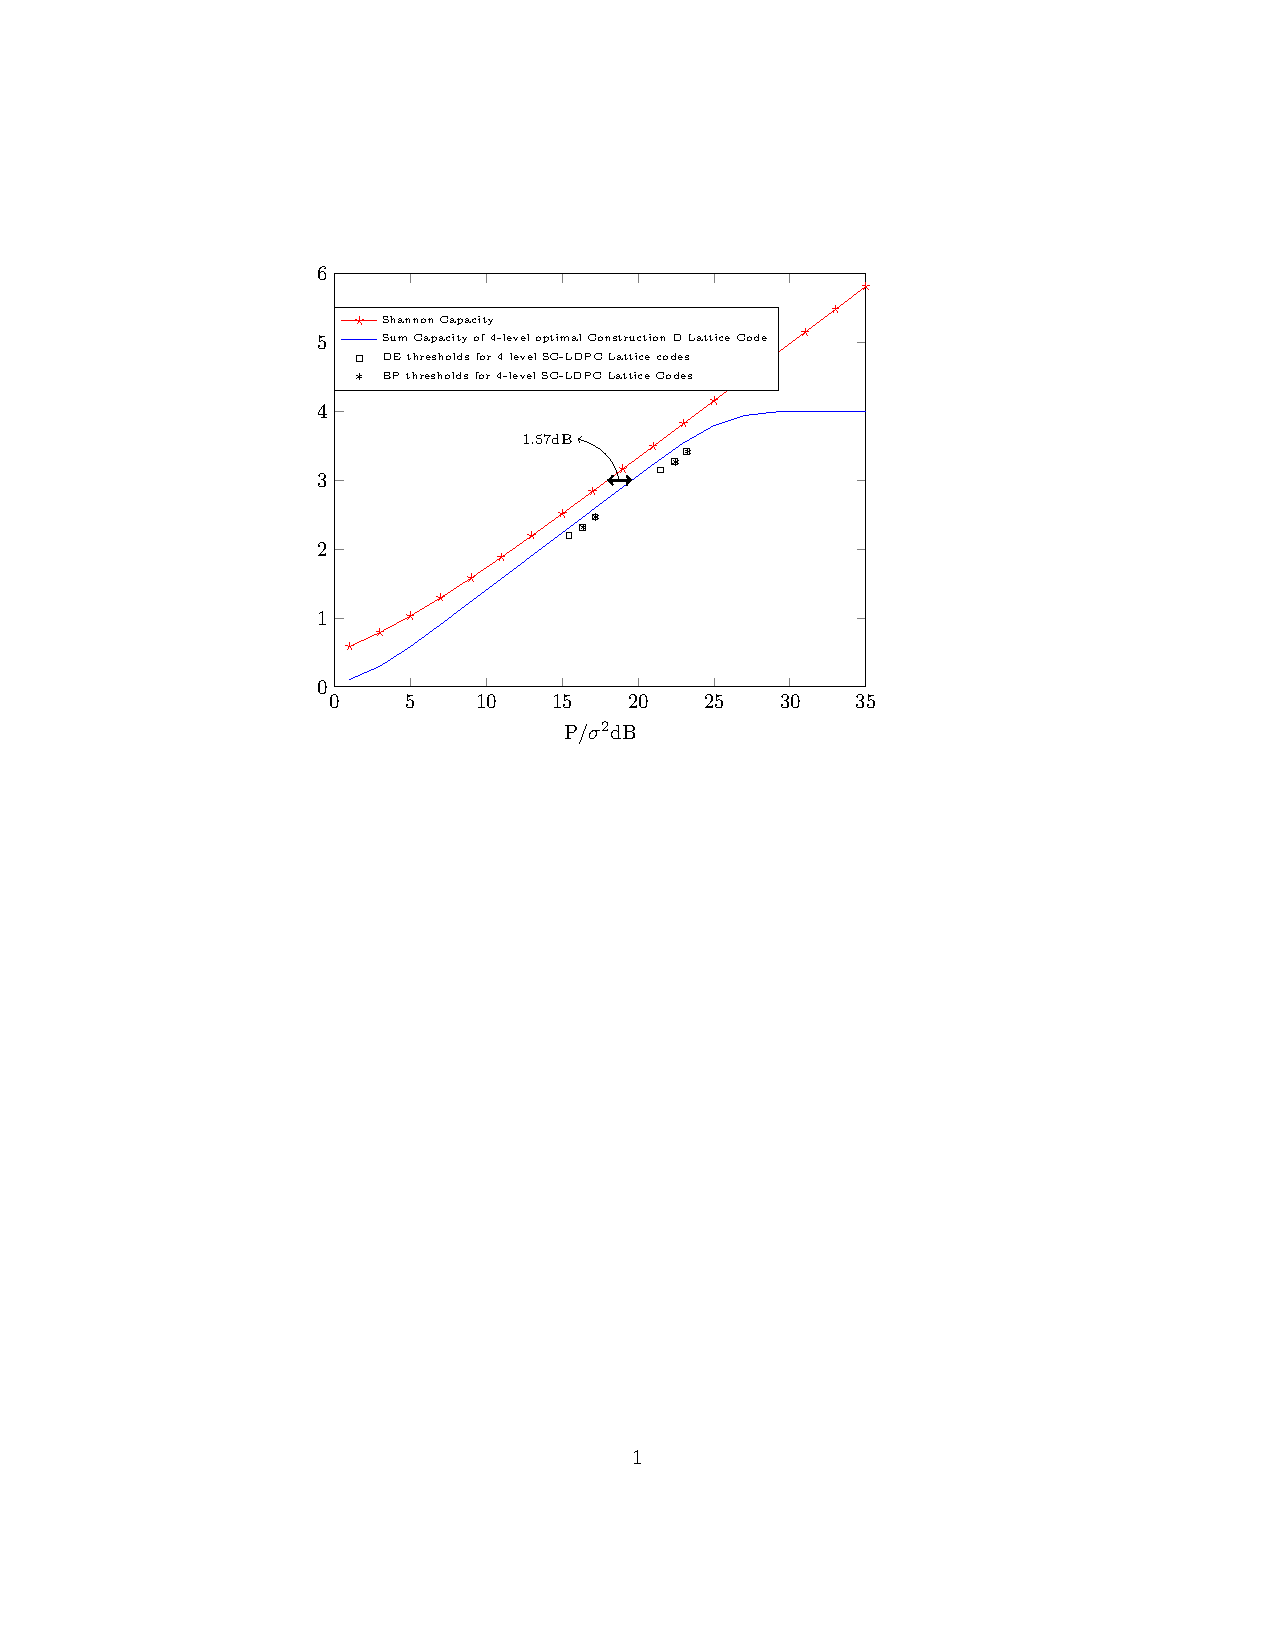
\includegraphics[width=2.75in]{\figpath/ShapingLoss_Final_CTW}
\end{frame}

%%---------------------------------------------------------------------------------------------------------------
%\begin{frame}\frametitle{Achievable Information Rates}
%    \begin{figure}
%        \begin{center}
%
%        \end{center}
%    \end{figure}
%\end{frame}

%%----------------------------------------------- DO NOT TOUCH-----------------------------------------------------------
%----------------------------------------------------------------------------------------------------------------------------------
\begin{frame}{Conclusion}
\begin{itemize} 
  \item Review of the peeling decoder
  \item Design of coding scheme with polynomial complexity for unsourced MAC with performance close to the random coding limit
  \item For the support recovery problem: coding scheme based on left and right regular Tanner graphs improving the sample and computational complexities matching the lower bound to a constant
    \item Improvement of testing and computational complexities for group testing using left and right Tanner graphs based design for the group testing problem. Improvement in testing complexity demonstrated for non-asymptotic regime
\end{itemize}
\end{frame}


%----------------------------------------------------------------------
\begin{frame}%\frametitle{Publications}
Preprints:
{\footnotesize 
\begin{itemize}
\item A. Vem, K. R. Narayanan, J. Cheng, J.-F. Chamberland, {\blue ``A User-Independent Serial Interference Cancellation Based Coding Scheme for the Unsourced Random Access Gaussian Channel",} to be published in ITW proceedings, 2017
\item A. Vem, N. T. Janakiraman, K. R. Narayanan,{\blue ``Group Testing using left-and-right-regular sparse-graph codes",} arXiv:1701.07477
\item N. T. Janakiraman, A. Vem, K. R. Narayanan, J.-F. Chamberland, ``Sub-string/Pattern Matching in Sub-linear Time Using a Sparse Fourier Transform Approach", arXiv:1704.07852
\end{itemize}
}

Conference:
{\footnotesize 
\begin{itemize}
\item A. Vem, N. T. Janakiraman, K. R. Narayanan, {\blue ``Sub-linear time compressed sensing for support recovery using left and right regular sparse-graph codes",} in Proc. of Information Theory Workshop, pp. 429-433, 2016
\item A. Taghavi, A. Vem, J.F. Chamberland, K.R. Narayanan, `` On the design of universal schemes for massive uncoordinated multiple access", in Proc. of International Symposium on Information Theory, pp. 345-349, 2016
\item S. Kumar, A. Vem, K. R. Narayanan, H. D. Pfister, ``Spatially-coupled codes for write-once memories", in Proc. of Annual Allerton Conference, pp. 125-131, 2015
\item S. Kumar, A. Vem, K. R. Narayanan, H. D. Pfister, ``Spatially-coupled codes for side-information problems", in Proc. of International Symposium on  Information Theory, pp. 516-520, 2014
\item A. Vem, Y. C. Huang, K. R. Narayanan, H. D. Pfister,  {\blue ``Multilevel lattices based on spatially-coupled LDPC codes with applications",} in Proc. of International Symposium on Information Theory, pp. 2336-2340, 2014
\end{itemize}
}
\end{frame}
%----------------------------------------------------------------------
\begin{frame}\frametitle{Questions?}
	\begin{figure}[t]
		\centering
		\includegraphics[width=2.8in]{\gt_figpath/questions}
	\end{figure}
	\centering
	\color{blue}
	\Huge{Thank you!}
\end{frame}

\end{document}